 %% 
%% Copyright 2019-2021 Elsevier Ltd
%% 
%% This file is part of the 'CAS Bundle'.
%% --------------------------------------
%% 
%% It may be distributed under the conditions of the LaTeX Project Public
%% License, either version 1.2 of this license or (at your option) any
%% later version.  The latest version of this license is in
%%    http://www.latex-project.org/lppl.txt
%% and version 1.2 or later is part of all distributions of LaTeX
%% version 1999/12/01 or later.
%% 
%% The list of all files belonging to the 'CAS Bundle' is
%% given in the file `manifest.txt'.
%% 
%% Template article for cas-sc documentclass for 
%% single column output.

\documentclass[a4paper,fleqnn]{cas-sc}

% If the frontmatter runs over more than one page
% use the longmktitle option.

%\documentclass[a4paper,fleqn,longmktitle]{cas-sc}

\hypersetup{colorlinks=true,allcolors=cyan}
\usepackage[numbers]{natbib}
%\usepackage[authoryear]{natbib}
%\usepackage[authoryear,longnamesfirst]{natbib}

%Cuong
\usepackage{amssymb}
\usepackage{latexsym}
\usepackage{amsmath}
\usepackage{dsfont}
\usepackage{amsfonts}
\usepackage{bigdelim}
%\usepackage[section]{placeins}
\usepackage{graphicx}
\usepackage{caption}
\usepackage{subcaption}
\captionsetup[subfloat]{labelformat=empty, font=footnotesize}
\usepackage{float}

%%%Author macros
\def\tsc#1{\csdef{#1}{\textsc{\lowercase{#1}}\xspace}}
\tsc{WGM}
\tsc{QE}
%%%

% Uncomment and use as if needed
%\newtheorem{theorem}{Theorem}
%\newtheorem{lemma}[theorem]{Lemma}
%\newdefinition{rmk}{Remark}
%\newproof{pf}{Proof}
%\newproof{pot}{Proof of Theorem \ref{thm}}

\begin{document}
\let\WriteBookmarks\relax
\def\floatpagepagefraction{1}
\def\textpagefraction{.001}

% Short title
\shorttitle{}    

% Short author
\shortauthors{D.C Hoang et al.}  

% Main title of the paper
\title [mode = title]{Multi-Scale Token Fusion with Mamba Adapters for Efficient 3D Industrial Defect Detection}  

% Title footnote mark
% eg: \tnotemark[1]
%\tnotemark[1] 

% Title footnote 1.
% eg: \tnotetext[1]{Title footnote text}
%\tnotetext[1]{tnote text} 

% First author
%
% Options: Use if required
% eg: \author[1,3]{Author Name}[type=editor,
%       style=chinese,
%       auid=000,
%       bioid=1,
%       prefix=Sir,
%       orcid=0000-0000-0000-0000,
%       facebook=<facebook id>,
%       twitter=<twitter id>,
%       linkedin=<linkedin id>,
%       gplus=<gplus id>]

\author[1]{Dinh-Cuong Hoang}[orcid=0000-0001-6058-2426]
\ead{cuonghd12@fe.edu.vn}
\cormark[1]

\author[2]{Phan Xuan Tan}
\ead{tanpx@shibaura-it.ac.jp}
\cormark[1]

\author[3]{Anh-Nhat Nguyen}
\ead{nhatna3@fe.edu.vn}

\author[1]{Duc-Huy Ngo}
\ead{huyndgch230154@fpt.edu.vn}
\author[1]{Minh-Duc Cao}
\ead{duccmgch230132@fpt.edu.vn}
\author[1]{Minh-Quang Vu}
\ead{quangvmgch230200@fpt.edu.vn}
\author[1]{Hoang-Nam Duong}
\ead{Dn6175j@gre.ac.uk}
\author[1]{Sy-Huong Nguyen}
\ead{huongnsgch230101@fpt.edu.vn}
\author[1]{Thi-Hong Le}
\ead{hongltgch230156@fpt.edu.vn}
\author[1]{Van-Viet Dang}
\ead{vietdvgbh230471@fpt.edu.vn}

\author[3]{Xuan-Tung Dinh}
\ead{tungdxhe172611@fpt.edu.vn}
\author[3]{Minh-Anh Nguyen}
\ead{anhnmhe182523@fpt.edu.vn}
\author[3]{Minh-Quang Do}
\ead{quangdmhe180854@fpt.edu.vn}
\author[3]{Van-Khanh Giap}
\ead{khanhgvhe176631@fpt.edu.vn}
\author[3]{Van-Hiep Duong}
\ead{hiepdvhe181185@fpt.edu.vn}


% Address/affiliation
\affiliation[1]{organization={Greenwich Vietnam, FPT University},
            city={Hanoi},
            postcode={10000}, 
            country={Vietnam}}

\affiliation[2]{organization={College of Engineering, Shibaura Institute of Technology},
            city={Tokyo},
            postcode={135-8548}, 
            country={Japan}}

\affiliation[3]{organization={ICT Department, FPT University},
            city={Hanoi},
            postcode={10000}, 
            country={Vietnam}}

\cortext[1]{Corresponding author}

% Footnote text
%\fntext[1]{}

% For a title note without a number/mark
%\nonumnote{}

% Here goes the abstract
\begin{abstract}
Three-dimensional (3D) industrial defect detection is critical for manufacturing quality assurance, robotic inspection, and safety-sensitive production environments, where reliable geometric anomaly localization directly impacts throughput and system reliability. However, 3D point clouds lack dense texture cues, exhibit unordered and irregular sampling, and offer limited annotated examples; as a result, many existing methods rely on handcrafted geometric descriptors or non-differentiable alignment heuristics that restrict scalability and generalization. We propose a novel 3D anomaly detection framework that integrates three complementary components: a Geometric Semantic-Aware Sorter (GSAS), a Mamba State-Space Adapter (MSSA), and an Attention-Based Discriminator (ABD). GSAS imposes a differentiable, surface-consistent soft-ordering of multi-layer per-patch tokens from a frozen pretrained Transformer; MSSA fuses these ordered tokens to propagate long-range, cross-layer context in linear time; and ABD localizes anomalies by producing slot-level logits that are reprojected to points for dense prediction. Evaluated on the synthetic Anomaly-ShapeNet and real-world Real3D-AD benchmarks using the area under the receiver operating characteristic (AUROC) metric, our method achieves 91.2\% and 76.6\% point-level AUROC respectively, surpassing the best compared baseline by +6.6\% and +2.8\%. The framework runs at approximately 17 frames per second (FPS) with a frozen Transformer backbone, establishing a new benchmark for efficient, interpretable 3D anomaly localization.
\end{abstract}


% Use if graphical abstract is present
%\begin{graphicalabstract}
%\includegraphics{}
%\end{graphicalabstract}

% Research highlights
%\begin{highlights}
%\item 
%\item 
%\item 
%\end{highlights}

% Keywords
% Each keyword is seperated by \sep
\begin{keywords}
 \sep Industrial anomaly detection \sep  Defect recognition \sep Object Anomaly Segmentation \sep
\end{keywords}

\maketitle

%%%%%%%%%%%%%%%%%%%%%%%%%%%%%%%%%%%%%%%%%%%%%%%%%%%%%%%%%%%%%%%%%%%%%%

\section{Introduction}

Industrial anomaly detection in the two-dimensional (2D) image domain has matured substantially over the last decade and provides a useful baseline for inspection tasks \cite{samrouth2025dual, casas2024comparative, liu2025improved}. Supervised and semi-supervised methods based on convolutional neural networks and transformer architectures achieve high detection accuracy when sufficient annotated defects are available \cite{venkataramanan2020attention,ding2022catching}. Unsupervised approaches, which train exclusively on defect-free images, have proven particularly practical: reconstruction-based models (autoencoders, GANs, diffusion systems) and feature-space methods (teacher-student distillation, memory banks, nearest-neighbor scoring) can localize diverse defect types without exhaustive annotations \cite{shi2021dfr,hou2021divide,zavrtanik2021draem,zavrtanik2022dsr,de2022masked,yao2023focus,defard2021padim,bergmann2020uninformed}. A complementary line of work synthesizes pseudo-anomalies in pixel or feature space (e.g., CutPaste, DRAEM, SimpleNet) to enable discriminative training from only normal samples \cite{li2021cutpaste,zavrtanik2021draem,liu2023simplenet}. These approaches benefit from dense photometric cues, regular grid structure, and a rich ecosystem of pretrained image encoders, which together simplify representation learning and spatial localization. Despite their practical success, purely 2D approaches have intrinsic limitations when applied to geometric defect detection. Photometric cues are unavailable or uninformative for many surface faults (e.g., subtle dents, thin cracks, or missing material) that primarily affect shape rather than appearance. Furthermore, 2D projections collapse 3D geometry and can hide defects through viewpoint or occlusion; compensating for this requires multi-view capture and careful alignment, which increases acquisition and processing complexity. Finally, feature distributions learned on natural images transfer imperfectly to industrial scans, producing domain shifts that reduce sensitivity to subtle, geometry-driven anomalies.

These limitations motivate direct anomaly analysis in three-dimensional (3D) data. Depth sensors and structured-light scanners provide point clouds and range maps that expose surface geometry, sampling density, and local curvature, which are essential for detecting geometry-only defects. Recent 3D methods exploit these cues using several strategies. Multimodal fusion approaches combine geometric descriptors with image-derived semantics to leverage complementary information\cite{cao2024complementary,wang2023multimodal,rudolph2023asymmetric}. Purely geometric pipelines operate directly on point clouds via teacher-student distillation, memory banks, registration, and prototype clustering to represent normal surface patterns \cite{bergmann2023anomaly,liu2023real3d,zhu2024towards}. Generative and self-supervised reconstruction models (masked reconstruction, diffusion-based denoising) learn to map anomalous inputs back to normal shapes and score deviations at the point level \cite{li2024towards,zhou2024r3d}. These directions demonstrate that 3D-specific cues substantially improve defect localization for shape-centric faults. However, existing 3D solutions exhibit several recurring limitations that impede robust, high-throughput deployment. First, many methods rely on handcrafted descriptors, large memory banks, costly registration or clustering procedures, or iterative generative inference; each increases runtime, memory footprint, or system complexity and thus complicates integration into production pipelines \cite{liu2023real3d,zhu2024towards}. Second, point clouds are unordered, irregularly sampled, and noisy, yet several approaches impose brittle, non-differentiable orderings or heuristic traversals to linearize geometry for sequence models; such orderings can mix distant surface regions and degrade context propagation \cite{liang2024pointmamba}. Third, reconstruction or input-space synthesis is sensitive to sampling artifacts and may inadvertently reconstruct defects, reducing anomaly contrast \cite{li2024towards,zhou2024r3d}. Fourth, the scarcity and narrow diversity of publicly available 3D anomaly benchmarks limit supervised fine-tuning and motivate synthetic or feature-space augmentation strategies, but the design of realistic pseudo-anomalies in 3D feature spaces remains under-explored. Finally, while large pretrained 3D backbones (e.g., masked point-cloud transformers) offer strong representations, most 3D anomaly methods either fine-tune them (incurring cost) or ignore cross-layer token structure (losing multi-scale cues); lightweight, differentiable adapters that preserve geometric locality are largely missing.

To address these challenges we propose a compact, practical framework\footnote{Code and dataset: \url{https://github.com/hoangcuongbk80/Mamba3dAD}} that combines geometry-preserving ordering, efficient sequential fusion, and localized discriminative scoring while leveraging large pretrained 3D Transformers with minimal backbone adaptation. First, we introduce a Geometric Semantic-Aware Sorter (GSAS), a differentiable soft-permutation that converts unordered multi-layer per-patch tokens into a spatially coherent ordered sequence; GSAS preserves local surface adjacency and produces contiguous surface trajectories that expose geometric structure to downstream sequence models. Second, we present Mamba, a linear-time state-space adapter that fuses the GSAS-ordered slots and propagates long-range, cross-layer context with minimal parameter and compute overhead, enabling contextual reasoning comparable to attention at substantially lower cost \cite{gu2021efficiently,gu2020hippo}. Third, an attention-based discriminator operates on the fused slot sequence and produces slot-level anomaly logits that are reprojected to points for dense localization. To train the discriminator without dense real-defect labels, we synthesize sparse pseudo-anomalies directly in the fused feature space; this feature-space corruption strategy yields localized supervisory signals that focus the model on discriminative deviations while preserving global shape priors. The resulting pipeline is compatible with frozen pretrained point cloud encoders, requires only lightweight adapter parameters, and scales to high-resolution scans.

Our method delivers substantial empirical gains while remaining computationally practical. On the synthetic Anomaly-ShapeNet benchmark we achieve a point-level AUROC of 91.2\% and AUPR of 38.7\%, and an object-level AUROC/AUPR of 86.8\%/98.7\%, improving over the strongest prior competitor (Group3AD) by 6.6\%  in point AUROC and 13.3\% in point AUPR. On the high-fidelity Real3D-AD scans we obtain a point-level AUROC of 76.6\% and AUPR of 19.7\%, and an object-level AUROC/AUPR of 78.4\%/77.7\%, exceeding Group3AD by 2.8\% and 5.8\% in point AUROC and AUPR, respectively. These gains are accompanied by practical runtime: the default configuration processes scans at roughly 17.3\,FPS, which is several times faster than reported runtimes of competing methods while preserving or improving localization accuracy. The results demonstrate that differentiable geometry-aware ordering plus efficient sequence fusion enables both state-of-the-art accuracy and the latency properties required for industrial inspection.

The main contributions of this paper are:
\begin{itemize}
  \item We propose a differentiable Geometric Semantic-Aware Sorter (GSAS) that produces spatially coherent soft-orderings of multi-layer 3D tokens, enabling sequence-modeling without sacrificing local surface fidelity.
  \item We introduce Mamba, a linear-time state-space adapter tailored to fuse ordered slot features and propagate long-range geometric context with low runtime and parameter overhead.
  \item We design an attention-based discriminator trained with sparse feature-space pseudo-anomalies to provide accurate point-level localization without requiring dense defect annotations.
  \item We validate the full pipeline on synthetic and real 3D anomaly benchmarks, demonstrating improved point- and object-level AUROC/AUPR over recent methods while maintaining practical inference speed suitable for deployment.
\end{itemize} 
%
\section{Related Work}
\label{sec:relatedwork}

\subsection{Industrial Image Anomaly Detection}

Industrial image anomaly detection (IAD) aims to identify and localize visual defects in manufacturing and inspection images. Prior research in this field can be broadly categorized according to the level of supervision available during training, namely supervised, semi-supervised, and unsupervised methods. Each category reflects a different trade-off between annotation cost, generalization ability, and detection performance.

Supervised methods formulate defect detection as a conventional classification or segmentation problem that relies on explicit anomaly annotations. Early approaches employ convolutional neural networks (CNNs) to learn discriminative representations of defective versus normal samples. Attention-based CNNs are designed to emphasize regions most relevant to defects \cite{venkataramanan2020attention}, while transformer architectures leverage their ability to capture long-range contextual dependencies for irregularity detection \cite{ding2022catching}. When sufficient labeled anomalies are available, supervised methods can achieve very high accuracy. However, collecting comprehensive labeled datasets that cover the wide diversity of defect types and appearance variations is often impractical in real industrial scenarios. As a result, these methods are limited by their dependence on exhaustive annotations.

Semi-supervised approaches attempt to bridge the gap between supervised and unsupervised paradigms by combining a small number of labeled anomalies with a large corpus of defect-free images. Common strategies include pseudo-labeling, class-imbalance reweighting, and hybrid pipelines that integrate unsupervised representation learning with supervised fine-tuning \cite{chadha2019comparison, chu2020neural}. For example, neural network adaptations can learn from sparse anomaly labels while preserving representations of normal data distributions. These methods often outperform purely unsupervised approaches when reliable anomaly labels exist. Nevertheless, their performance still heavily depends on the diversity and quality of the labeled anomalies, and it tends to degrade when anomalies exhibit substantial variation or unseen patterns.

Unsupervised IAD methods eliminate the need for anomaly annotations entirely. They are trained exclusively on defect-free images and are designed to detect anomalies by identifying deviations from learned normal patterns during inference. Two main paradigms dominate this category. The first focuses on reconstruction-based learning, where models such as autoencoders, generative adversarial networks (GANs), diffusion models, and vision transformers are trained to reconstruct normal samples under the assumption that defects will result in higher reconstruction errors. Representative examples include multi-scale feature-guided autoencoders \cite{shi2021dfr}, divide-and-assemble memory-based models \cite{hou2021divide}, joint reconstruction–discrimination embeddings \cite{zavrtanik2021draem}, and dual subspace re-projection (DSR) \cite{zavrtanik2022dsr} that simulates near-in-distribution defects. Recently, diffusion and transformer-based inpainting frameworks such as masked transformers \cite{de2022masked}, dual attention architectures \cite{yao2023focus}, adaptive inpainting networks (AMI-Net) \cite{luo2024ami}, and dynamic diffusion systems \cite{zhang2023unsupervised, lu2023removing, tebbe2024dynamic} have further improved reconstruction fidelity and localization precision. Although these approaches are conceptually simple and widely applicable, they require careful architectural design and regularization to prevent over-smoothing or the unintended reconstruction of defects.

The second major family of unsupervised methods operates in feature space rather than pixel space. These methods rely on pretrained visual encoders to extract semantic embeddings of normal images and then measure deviations from these embeddings during testing. Teacher–student distillation frameworks train a student network to imitate the feature representations of a fixed teacher model, where large deviations between the two networks indicate potential anomalies \cite{bergmann2020uninformed, salehi2021multiresolution, wan2022unsupervised, gu2023remembering, tong2024enhanced}. Memory-based approaches maintain a feature bank of representative normal descriptors and identify anomalies using nearest-neighbor search or probabilistic distance metrics \cite{defard2021padim, roth2022towards, bae2023pni, zuo2024reconstruction, hyun2024reconpatch}. These feature-based methods benefit from the semantic richness of large pretrained models but are sensitive to domain shift, since industrial imagery often differs substantially from natural images such as those in ImageNet. As a consequence, mismatched feature distributions can limit anomaly sensitivity in industrial applications.

A complementary research direction focuses on synthesizing pseudo-anomalies to enable discriminative training without requiring true defect labels. Pixel-level anomaly generation methods such as CutPaste \cite{li2021cutpaste} and discriminative synthetic augmentation frameworks \cite{zavrtanik2021draem} create artificial anomalies on clean images and train a classifier to distinguish between the original and augmented samples. While simple and efficient, these pixel-space synthesis techniques often fail to match the visual and semantic characteristics of real industrial defects. Recent work addresses this limitation by synthesizing anomalies directly in the feature space or by adapting pretrained networks to the target domain. For instance, feature adaptors fine-tune pretrained CNNs to reduce domain bias and improve the relevance of anomaly signals \cite{liu2023simplenet}. Other approaches generate near-in-distribution perturbations that better approximate realistic defect patterns \cite{zavrtanik2022dsr, fang2023fastrecon, zhang2024realnet}.

Despite these advances, several open challenges remain. The most prominent include achieving representations that are both discriminative for subtle local defects and robust under domain shift, generating realistic synthetic anomalies that provide meaningful supervision, and designing architectures that balance detection accuracy with real-time efficiency. Addressing these challenges motivates recent hybrid approaches that integrate geometry-aware representation learning, efficient context aggregation, and realistic feature-space anomaly synthesis, which form the foundation for our proposed method.

\subsection{Industrial 3D Anomaly Detection}

Anomaly detection in three-dimensional (3D) data is an emerging research area that complements the more mature literature on two-dimensional (2D) methods \cite{horwitz2023back}. Depth sensors provide rich geometric and structural cues that can improve defect localization and diagnosis, but they also impose unique algorithmic and practical challenges. Recent work has addressed these opportunities and challenges using multimodal fusion, purely geometric reasoning, self-supervised reconstruction, and generative denoising paradigms.

One line of work combines geometric descriptors with image-based semantic cues to leverage complementary modalities. The Complementary Pseudo Multimodal Feature (CPMF) framework integrates handcrafted local point cloud features with global semantic information obtained from pseudo-view projections processed by pretrained networks \cite{cao2024complementary}. Related multimodal methods fuse geometric and photometric information to increase robustness under varying capture conditions and to improve localization accuracy \cite{wang2023multimodal, rudolph2023asymmetric}. These approaches exploit the strengths of both modalities, but they may depend on careful alignment between 2D and 3D domains and on the availability of reliable color or intensity channels.

A second category focuses on methods that operate directly in the 3D domain and that therefore avoid cross-modal alignment issues. The 3D Student-Teacher method (3D-ST) extended the student–teacher paradigm to point clouds and demonstrated that a student trained to imitate a self-supervised teacher can localize geometric anomalies with a single forward pass \cite{bergmann2023anomaly}. Registration- and memory-based schemes, such as Reg3D-AD, combine raw coordinates with learned features from masked point cloud encoders (for example PointMAE) to build neighborhood-sensitive memory banks that represent normal geometry \cite{liu2023real3d}. Group3AD represents anomalies with group-level feature prototypes and enforces inter-cluster uniformity and intra-cluster alignment to improve discriminability \cite{zhu2024towards}. These geometric approaches remove dependencies on image-based cues and can provide fine-grained localization, but several such methods incur substantial computational and memory overhead due to large memory banks, registration steps, or complex clustering procedures.

Self-supervised reconstruction and generative models form a third family of approaches for 3D anomaly detection. IMRNet uses iterative mask reconstruction with geometry-aware sampling to preserve potentially anomalous structures during downsampling and employs a transformer to reconstruct masked patches in a self-supervised manner \cite{li2024towards}. R3D-AD adopts a diffusion-based reconstruction strategy that learns point-wise displacements to convert anomalous inputs into their normal counterparts \cite{zhou2024r3d}. These generative methods can produce high-fidelity reconstructions and enable pixel- or point-level anomaly scoring, but they typically require iterative inference, careful regularization, and substantial compute to achieve stable results.

Despite these advances, practical deployment in industrial settings remains challenging. First, many state-of-the-art 3D methods are computationally intensive or memory hungry, which complicates integration into production inspection pipelines that require high throughput. Second, publicly available 3D anomaly datasets are limited in scale and diversity, and this scarcity of labeled anomalies places a premium on robust self-supervised and synthetic-augmentation strategies. Third, real-world data often exhibits occlusion, variable sampling density, and sensor noise, all of which can confound methods that assume well-behaved geometric inputs. These limitations motivate designs that explicitly address computational efficiency, domain adaptation, and robustness to capture artifacts.

Motivated by the simplicity and efficiency of SimpleNet in the 2D setting \cite{liu2023simplenet}, we aim to develop an equally compact and practical architecture for 3D point cloud anomaly detection. Directly adapting SimpleNet to point clouds is not straightforward because point clouds are unordered and irregular, and because they require permutation-invariant operations and explicit modeling of local geometric relationships. In addition, 3D scans present higher dimensionality, variable point density, and sensor noise that demand specialized feature extraction and domain adaptation. To address this we ...

\subsection{State Space Model}

State-space models (SSMs) formulate sequence processing as learned linear dynamical systems and have recently been adapted into neural layers for long-range dependency modeling \cite{gu2020hippo,gu2021efficiently,gu2021combining,gu2022parameterization,smith2022simplified}.  Early foundational work introduced HiPPO-style projection frameworks that give principled recurrent memory for very long horizons \cite{gu2020hippo}.  Building on these ideas, the Structured State Space for Sequence modeling (S4) family exploited algebraic structure and frequency-domain computation to make deep SSMs both expressive and efficient on long-horizon benchmarks \cite{gu2021efficiently}.  Follow-up studies improved practical usability by reparameterizing layers, adopting multi-input multi-output constructions, and stabilizing initialization so that SSM layers can be trained in parallel and at scale \cite{gu2021combining,gu2022parameterization,smith2022simplified}.

Parallel to advances in attention and convolutional architectures, researchers have investigated how SSM blocks can serve as alternatives or complements in vision pipelines.  Compared to self-attention-based transformers \cite{vaswani2017attention}, SSM layers can offer lower memory footprints and near-linear runtime when applied to long token sequences, which is attractive for high-resolution inputs.  Recent papers adapt the basic SSM toolkit to two-dimensional signals by converting images or feature maps into ordered token streams, adding positional encodings, and designing bidirectional or multi-scale scans to recover spatial context \cite{zhu2024vision,liu2024vmamba,guo2024mambair}.  These vision-focused adaptations report competitive results on classification and restoration tasks while reducing per-batch memory and speeding throughput in many settings \cite{zhu2024vision,liu2024vmamba,guo2024mambair}.

SSM-driven designs have also been extended to geometric and low-level vision problems.  For image restoration, lightweight SSM variants applied on multi-scale features achieve good fidelity-versus-latency trade-offs by exploiting the linear recurrence to propagate information across large receptive fields.  For point-cloud processing, several works linearize spatial neighborhoods using carefully chosen traversal orders and then apply SSM modules to capture long-range geometric relationships; additional local aggregation or constrained parameterizations are used to preserve fine-grained geometry \cite{liang2024pointmamba,han2024mamba3d,zha2024lcm}.  These studies demonstrate that state-space layers are versatile primitives that can be tailored to both dense pixel-level tasks and irregular 3D data.

Our contribution is complementary to these lines of work.  Rather than replacing pretrained visual backbones or retraining large models from scratch, we design a compact, parameter-efficient adapter that embeds Mamba-style SSM processing into intermediate stages of an off-the-shelf backbone.  The adapter fuses cross-stage representations and propagates long-range context with little extra compute, enabling improved feature integration while keeping the backbone weights frozen.  In this way, our proposal bridges algorithmic advances in SSMs and practical, low-cost integration into large-scale vision systems.
 

%
\section{Methodology}

\begin{figure}[h!]
  \centering 
    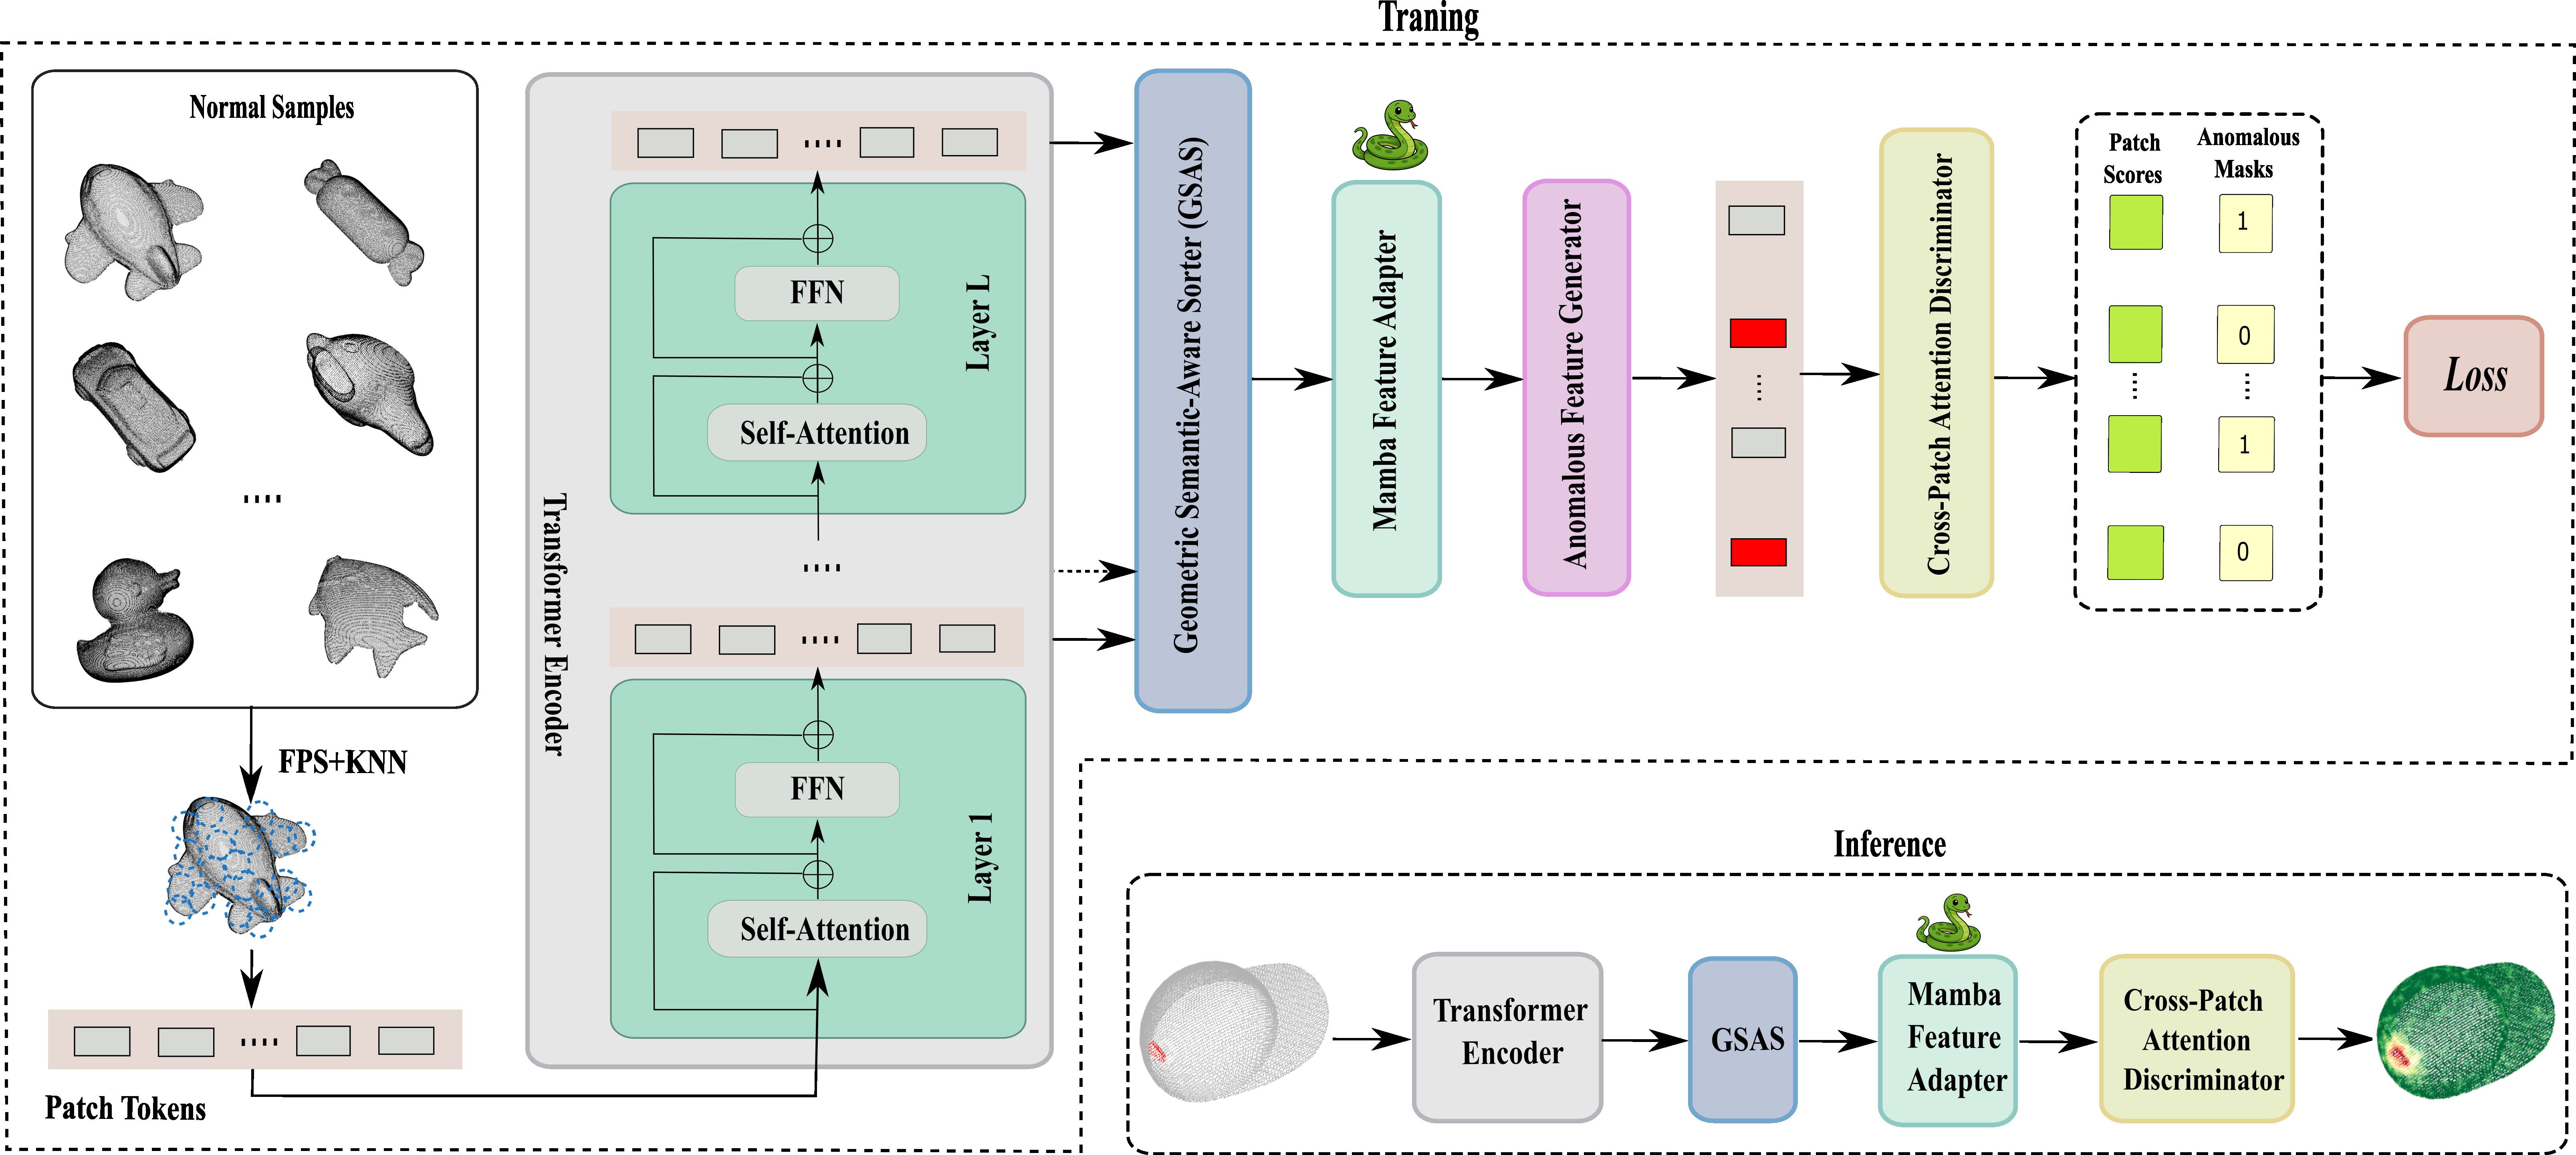
\includegraphics[width=0.98\linewidth]{figs/overview}
  \caption{Overview of the proposed 3D anomaly detection pipeline.}
  \label{fig:overview}
\end{figure}

We address efficient 3D anomaly detection that requires minimal task-specific training while preserving geometric structure and long-range contextual reasoning. As illustrated in Figure \ref{fig:overview}, given an input point cloud \(\mathcal{P} = \{\mathbf{p}_i \in \mathbb{R}^3\}_{i=1}^N\), the proposed pipeline leverages a frozen pre-trained point-cloud Transformer together with a compact set of lightweight adapters to generate spatially coherent and anomaly-sensitive representations. The backbone consists of \(L\) encoder layers, each producing \(M\) patch tokens of dimension \(D\); we denote the patch-token matrix and class token at layer \(i\) as \(\mathbf{T}_i \in \mathbb{R}^{M\times D}\) and \(c_i \in \mathbb{R}^{1\times D}\), respectively, and collect the hierarchical token set \(\mathbf{T} = \{\mathbf{T}_1, \dots, \mathbf{T}_L\}\) with a total of \(T = L \cdot M\) tokens. These unordered layer-wise tokens are transformed into a semantically ordered sequence \(\mathbf{T}_{\mathrm{ord}} \in \mathbb{R}^{T\times D}\), subsequently fused into enriched contextual features \(y_{1:T} \in \mathbb{R}^{T\times D}\), and finally scored by a lightweight attention-based discriminator for per-patch anomaly localization. The geometric semantic-aware sorter (GSAS) establishes a differentiable soft-permutation that orders the hierarchical tokens while preserving geometric locality and semantic consistency. The Mamba adapter, a linear-time state-space model, efficiently fuses the ordered sequence to yield context-enhanced features \(y_{1:T}\) that retain both local fidelity and global awareness. A selective anomaly generator operates during training to inject sparse feature-space perturbations, enabling effective supervision without real defect labels. The cross-patch discriminator then aggregates contextual cues through a compact attention mechanism to output patch-level anomaly logits, which are reprojected to points for precise localization. 

\subsection{Backbone}

Given an input point cloud \(\mathcal{P} = \{\mathbf{p}_i\in\mathbb{R}^3\}_{i=1}^N\), the backbone produces local patch embeddings and a hierarchical set of Transformer tokens that preserve patch identities across layers. We apply Farthest Point Sampling (FPS) to select \(M\) patch centers \(\{p_j\in\mathbb{R}^3\}_{j=1}^M\), where index \(j\) denotes a patch center, and for each center we collect a fixed-size neighborhood of \(K\) points via \(K\)-nearest neighbors (KNN). Each neighborhood is embedded by a lightweight PointNet encoder followed by a positional-encoding MLP to yield an initial patch embedding \(x_j^{(0)}\in\mathbb{R}^D\), for \(j=1,\dots,M\). The \(M\) initial embeddings are concatenated with a global class token \(c_0\in\mathbb{R}^{1\times D}\) to form the Transformer input \([c_0;\mathbf{T}_0]\), where \(\mathbf{T}_0=[x_1^{(0)};\dots;x_M^{(0)}]\in\mathbb{R}^{M\times D}\). These are passed to the frozen Point-MAE Transformer pretrained on ShapeNet~\cite{pang2022masked,chang2015shapenet}. Formally, the \(i\)-th Transformer block \(\ell_i(\cdot)\) computes
\begin{equation}
[c_i;\,\mathbf{T}_i] \;=\; \ell_i([c_{i-1};\,\mathbf{T}_{i-1}]), \qquad i=1,\dots,L,
\end{equation}
with \(\mathbf{T}_i=[t_{i,1};\dots;t_{i,M}]\in\mathbb{R}^{M\times D}\) and \(c_i\in\mathbb{R}^{1\times D}\). The spatial coordinates \(\{p_j\}\) remain associated with their patch index \(j\) and are reused at every Transformer layer; consequently token \(t_{i,j}\) at layer \(i\) corresponds to the same geometric patch center \(p_j\). The backbone therefore outputs the initial patch embeddings \(\{x_j^{(0)}\}_{j=1}^M\) with \(x_j^{(0)}\in\mathbb{R}^D\), the hierarchical tokens \(\{\mathbf{T}_i\}_{i=1}^L\) with \(\mathbf{T}_i\in\mathbb{R}^{M\times D}\), the sequence of class tokens \(\{c_i\}_{i=1}^L\) with \(c_i\in\mathbb{R}^{1\times D}\), and the retained patch centers \(\{p_j\}_{j=1}^M\in\mathbb{R}^3\). Optionally, these tokens may be viewed as a flattened set \(\mathbf{T}=\{\mathbf{T}_1,\dots,\mathbf{T}_L\}\) of \(T=L\cdot M\) tokens in \(\mathbb{R}^{T\times D}\).

\subsection{Geometric Semantic-Aware Sorter (GSAS)}
\label{sec:gsas}

\begin{figure}[h!]
  \centering 
    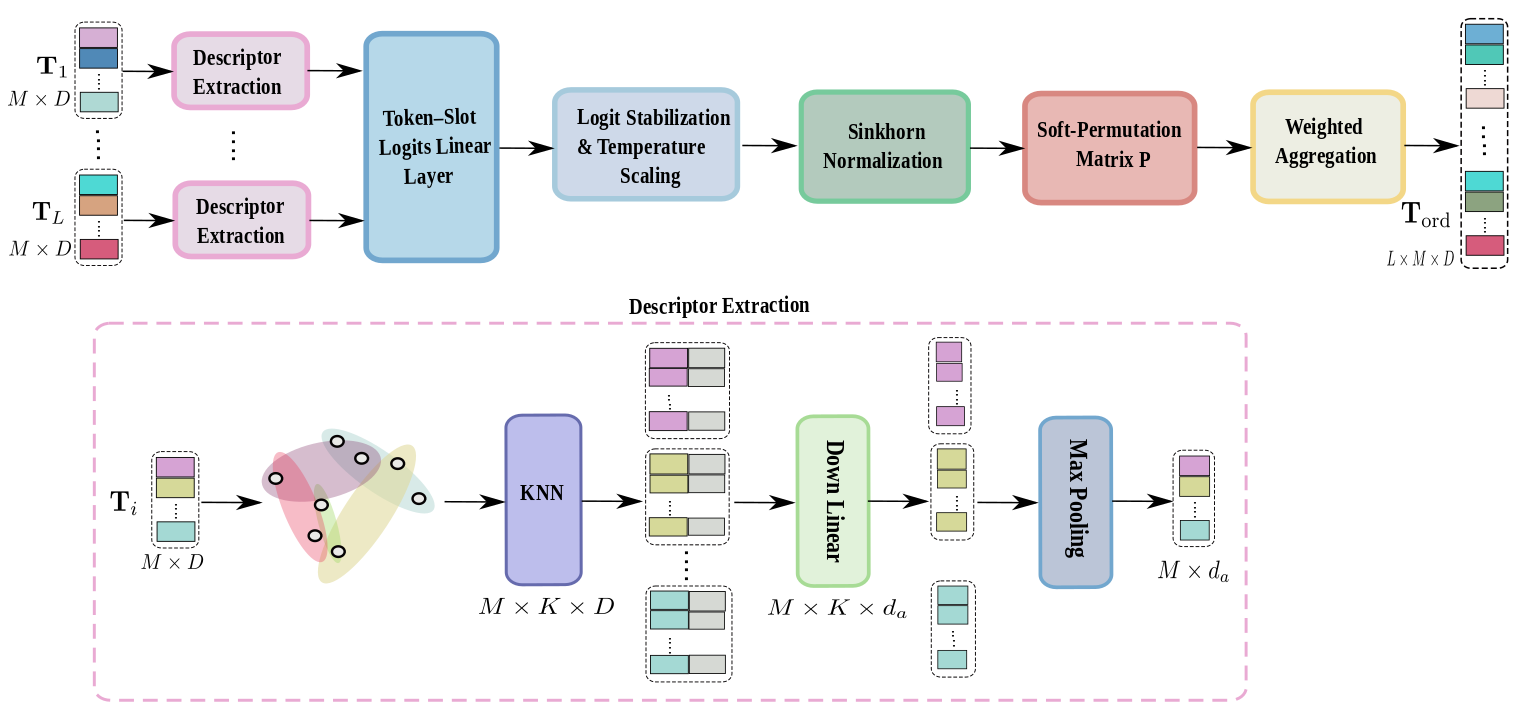
\includegraphics[width=0.98\linewidth]{figs/GSAS}
  \caption{Overview of geometric semantic-aware sorter (GSAS).}
  \label{fig:GSAS}
\end{figure}

Given input tokens \(X\in\mathbb{R}^{T\times D}\), where \(X\) denotes the flattened collection of all per-layer tokens \(t_{i,j}\) produced by the backbone (so that each \(\mathbf{T}_i=[t_{i,1};\dots;t_{i,M}]\in\mathbb{R}^{M\times D}\) and \(T=L\cdot M\)), and given the unique patch centers \(\{p_j\in\mathbb{R}^3\}_{j=1}^M\), GSAS produces a differentiable ordering of the \(T\) tokens that preserves local surface adjacency and semantic affinity. As illustrated in Figure ~\ref{fig:GSAS}, we first summarizes local geometry and same-layer semantics, then computes token-slot affinities, converts affinities to an approximately doubly-stochastic assignment, and finally aggregates tokens into ordered slots for downstream fusion.

We construct a kNN graph on the unique patch centers and denotes the neighbor set of patch \(j\) by \(\mathcal{N}_{\mathrm{patch}}(j)\subset\{1,\dots,M\}\). For a token \(t\) corresponding to \((i,j)\) with \(i=i(t)\) and \(j=j(t)\), GSAS computes a permutation-invariant local descriptor by aggregating features from the same Transformer layer \(i\) of neighboring patches:
\begin{equation}
u_{i,j} \;=\; \mathrm{MaxPool}\Big(\big\{\,W_{\downarrow}\,t_{i,u} + b_{\downarrow} \ \big|\ u\in\mathcal{N}_{\mathrm{patch}}(j)\big\}\Big)\in\mathbb{R}^{d_a},
\end{equation}
where \(W_{\downarrow}\in\mathbb{R}^{d_a\times D}\) and \(b_{\downarrow}\in\mathbb{R}^{d_a}\). The module collects these descriptors into \(E\in\mathbb{R}^{T\times d_a}\) by setting \(E_{t,:}=u_{i(t),j(t)}\). The descriptor \(E\) summarizes local geometry while preserving layer-specific semantics, and GSAS uses \(E\) to inform the affinity computation in the next step. We computes raw token-slot affinities from the descriptors:
\begin{equation}
\mathbf{G} \;=\; E\,W_{\uparrow} + \mathbf{1}\,b_{\uparrow}^\top \in\mathbb{R}^{T\times T},
\end{equation}
with \(W_{\uparrow}\in\mathbb{R}^{d_a\times T}\), \(b_{\uparrow}\in\mathbb{R}^T\), and \(\mathbf{1}\in\mathbb{R}^{T\times 1}\). The matrix \(\mathbf{G}\) encodes unnormalized affinities between tokens and ordered slots, and GSAS processes \(\mathbf{G}\) to produce a differentiable assignment that can be optimized end-to-end.

For numerical stability we subtract the column-wise maximum \(v\in\mathbb{R}^T\) with entries \(v_s=\max_t \mathbf{G}_{t,s}\), applies temperature scaling and exponentiation, and normalizes with the Sinkhorn operator:
\begin{equation}
\tilde{\mathbf{G}} \;=\; (\mathbf{G} - \mathbf{1}\,v^\top)/\tau,
\end{equation}
\begin{equation}
P \;=\; \mathrm{Sinkhorn}\big(\exp(\tilde{\mathbf{G}}),\,K_{\mathrm{sink}}\big)\in[0,1]^{T\times T},
\end{equation}
where \(\tau>0\) denotes the temperature and \(K_{\mathrm{sink}}\) the number of iterations. The soft-permutation \(P\) is approximately doubly-stochastic and differentiable, and GSAS uses \(P\) to aggregate token features into a semantically coherent ordered sequence. We aggregate tokens into ordered slots by weighted summation:
\begin{equation}
\mathbf{T}_{\mathrm{ord}} \;=\; P^\top X \in\mathbb{R}^{T\times D},
\end{equation}
\begin{equation}
\mathbf{T}_{\mathrm{ord}}[s,:]=\sum_{t=1}^T P_{t,s}\,X_t.
\end{equation}
The aggregation yields one feature vector per ordered slot while preserving differentiability so that gradients propagate to \(W_{\downarrow},b_{\downarrow},W_{\uparrow},b_{\uparrow}\). The ordered tokens \( \mathbf{T}_{\mathrm{ord}}\) therefore provide the contiguous, semantically coherent input required by the subsequent fusion module.

We include two auxiliary regularizers to prevent degenerate assignments and to encourage geometric locality. The column-wise entropy penalty discourages diffuse assignments into a given slot:
\begin{equation}
\mathcal{L}_{\mathrm{ent}} \;=\; \frac{1}{T}\sum_{s=1}^T H(P_{:,s}),\qquad
H(\pi)=-\sum_{t}\pi_t\log(\pi_t+\epsilon_{\mathrm{ent}}),
\end{equation}
with \(\epsilon_{\mathrm{ent}}>0\) for numerical stability. The entropy penalty directly biases the columns of \(P\) toward concentrated assignments and thus improves the quality of aggregation in Eq. for \(\mathbf{T}_{\mathrm{ord}}\). The locality penalty measures expected slot positions \(\mu_t\) and biases them to align with geometric affinities:
\begin{equation}
\mu_t \;=\; \sum_{s=1}^T \tilde s\,P_{t,s}\in[0,1],
\end{equation}
\begin{equation}
w_{t,u} \;=\; \exp\!\big(-\|p_{j(t)}-p_{j(u)}\|^2/\sigma_p^2\big),
\end{equation}
\begin{equation}
\mathcal{L}_{\mathrm{loc}} \;=\; \sum_{t=1}^T \frac{1}{\sum_{u=1}^T w_{t,u} + \epsilon_{\mathrm{norm}}}\sum_{u=1}^T w_{t,u}\,\big(\mu_t - \mu_u\big)^2,
\end{equation}
where \(\tilde s=(s-1)/\max(1,T-1)\), \(\sigma_p\) is a bandwidth parameter, and \(\epsilon_{\mathrm{norm}}>0\) stabilizes the normalization. The locality penalty directly influences \(\mu_t\) and thus biases the soft-permutation \(P\) to place geometrically adjacent tokens into nearby slots.

\subsubsection{Mamba Feature Adapter}

After GSAS produces the ordered token matrix $\mathbf{T}_{\mathrm{ord}}\in\mathbb{R}^{T\times D}$, let the row-wise sequence be
$$
x_{1:T},\qquad x_t=\mathbf{T}_{\mathrm{ord}}[t,:]\in\mathbb{R}^D,\quad t=1,\dots,T.
$$
The Mamba adapter is formulated as a state-space model that fuses long-range, layer-wise context along the GSAS-induced ordering. Let the latent dimension be $S$. The recurrence and output equations are defined as
\begin{equation}
h_t = A\,h_{t-1} + B\,x_t,\qquad h_0=\mathbf{0}\in\mathbb{R}^S,
\end{equation}
\begin{equation}
\tilde{q}_t = C\,h_t + D\,x_t \in\mathbb{R}^D,
\end{equation}
where
$$
A\in\mathbb{R}^{S\times S},\quad 
B\in\mathbb{R}^{S\times D},\quad 
C\in\mathbb{R}^{D\times S},\quad 
D\in\mathbb{R}^{D\times D}.
$$
The sequence of adapted outputs is collected as
$$
Q=[\tilde{q}_1,\dots,\tilde{q}_T]^\top\in\mathbb{R}^{T\times D},
$$
and, for consistency with the subsequent modules, $q_t\equiv\tilde{q}_t$.

The GSAS module determines the sequence order $x_{1:T}$, while the Mamba adapter performs contextual integration along this induced order without altering the token arrangement. The parameters $\{A,B,C,D\}$ are shared across all time steps, ensuring parameter efficiency and preserving the linear computational complexity with respect to sequence length $T$. Specifically, Mamba operates in $\mathcal{O}(T)$ time and requires $\mathcal{O}(S)$ additional memory per step, in contrast to the $\mathcal{O}(T^2)$ cost of full self-attention. The residual term $D\,x_t$ maintains per-token fidelity, while $C\,h_t$ introduces long-range contextual dependencies through the recurrent hidden state. The Mamba parameters are optimized jointly with the GSAS parameters, positional MLP, anomaly-scaling $\gamma$, and discriminator weights, whereas the Transformer backbone remains frozen.

\subsection{Anomalous Feature Generator}
Industrial defects in 3D point clouds are typically sparse, subtle, and spatially localized. To simulate such defects during training without requiring external anomaly examples, we introduce a lightweight, selective feature-space perturbation that synthesizes pseudo-anomalous tokens by injecting noise into a sparse subset of adapted token embeddings. Given output from Mamba feature adapter $Y$.

We sample an independent Bernoulli mask per token to determine corruption:
\begin{equation}
m_t \sim \mathrm{Bernoulli}(p),\qquad m_t\in\{0,1\},
\end{equation}
where \(p\in(0,1)\) controls expected corruption sparsity and is selected on validation (to reflect realistic, sparse defect rates we typically choose \(p\ll 0.5\) and tune it on held-out data). When \(m_t=1\) the token is corrupted by an additive isotropic Gaussian perturbation in the canonical token space:
\begin{equation}
\varepsilon_t \sim \mathcal{N}\big(0,\sigma^2 I_D\big),
\end{equation}
where \(\sigma>0\) controls perturbation scale (we validate \(\sigma\); a practical value is \(\sigma=0.1\)). The pseudo-anomalous token is defined as
\begin{equation}
\tilde{q}_t \;=\; q_t + \gamma\, m_t\, \varepsilon_t,
\end{equation}
where \(\gamma\ge 0\) is a learnable scalar that adaptively rescales the injected perturbation (initialized to a small positive value). When \(m_t=0\) we have \(\tilde{q}_t=q_t\). This corruption mechanism is applied only during training; at inference time the generator is disabled (\(m_t\equiv 0\)) and all tokens remain clean.

The selective (sparse) corruption contrasts with indiscriminate global noise: by corrupting a small fraction of slots we emulate localized defects while preserving the normal manifold for the majority of features. Because sparse corruption can induce class imbalance, we (i) recommend validating \(p\) on held-out data and (ii) mitigate imbalance via weighted loss or controlled sampling (details in the training section).

\subsection{Cross-Patch Attention Discriminator}
Detecting defects often requires contextual comparison across patches. We therefore employ a lightweight attention-based discriminator that jointly processes all patch slots and outputs a scalar logit per slot. To preserve spatial information and to generalize across varying patch arrangements, positional embeddings are derived from patch center coordinates rather than learned per-slot indices. Let \(p_t\in\mathbb{R}^3\) denote the patch center associated with slot \(t\); the positional embedding is computed by a small coordinate MLP:
\begin{equation}
e_t \;=\; \mathrm{PE\text{-}MLP}(p_t) \in\mathbb{R}^D.
\end{equation}

During training we construct a single mixed input sequence for the discriminator in which corrupted tokens replace clean tokens in-place. The discriminator input for slot \(t\) is therefore
\begin{equation}
\hat{q}_t \;=\; \big(m_t\,\tilde{q}_t + (1-m_t)\,q_t\big) + e_t \;=\; q_t + m_t(\gamma\varepsilon_t) + e_t,
\end{equation}
and the supervision label is \(y_t=m_t\). Inference uses the same pipeline but with \(m_t\equiv 0\) so that \(\hat{q}_t=q_t+e_t\).

Let \(H\) denote the number of attention heads and \(d_{\mathrm{head}}=D/H\) the per-head dimension; in practice we choose \(D\) divisible by \(H\) or insert a thin linear projection to meet this constraint. The discriminator applies a single multi-head self-attention layer followed by a compact shared MLP head that maps each token to a scalar logit:
\begin{align}
Z \; &=\; \mathrm{MHA}(\{\hat{q}_t\}_{t=1}^T)\in\mathbb{R}^{T\times D},\\
s_t \; &=\; \mathrm{MLP}_{\mathrm{head}}(Z_t)\in\mathbb{R}.
\end{align}
Here \(\mathrm{MHA}(\cdot)\) denotes standard multi-head self-attention with appropriate query/key/value projections, scaled dot-product attention, residual connections, dropout and layer normalization; \(\mathrm{MLP}_{\mathrm{head}}\) is a two-layer feedforward network (one hidden layer) shared across slots and producing a scalar logit. Layer normalization and dropout are included to stabilize training. Because the discriminator processes all tokens jointly, each output \(s_t\) reflects both local evidence and global context, improving sensitivity to structured or context-dependent defects compared to independent per-slot scoring.

At test time the discriminator receives only clean tokens \(\{q_t\}\) augmented with positional embeddings \(e_t\) and outputs per-slot logits \(s_t\). These per-slot scores are reprojected to the original point cloud by assigning each point the maximal score of the patches that contain it (see Inference section).

\subsection{Loss Function and Training}
\label{sec:loss}

We jointly optimize the trainable components (GSAS parameters, Mamba adapter parameters, positional-embedding MLP, the anomaly-scaling \(\gamma\), and discriminator parameters) using a patch-wise binary classification objective. Let \(\Theta\) denote the set of all trainable parameters. For a training batch we accumulate \(P\) supervised token slots (summed across batch and sequence). We use a numerically-stable logits-based binary cross-entropy implemented as BCE-with-logits. The per-slot logits-based loss (stable form) is:
\begin{equation}
\ell_{\mathrm{BCElogits}}(s,y) \;=\; \max(s,0) - s\,y + \log\big(1+\exp(-|s|)\big),
\end{equation}
and the unweighted batch loss is \(\mathcal{L}_{\mathrm{BCE}}=\frac{1}{P}\sum_{t=1}^P \ell_{\mathrm{BCElogits}}(s_t,y_t)\). To mitigate class imbalance when corruption is sparse we optionally use a positive-class weighting factor \(w_+>0\) (e.g., \(w_+=(1-p)/p\) or a value tuned on validation) via the standard \texttt{pos\_weight} mechanism of BCE-with-logits; this multiplies the contribution of positive (corrupted) examples.

We complement \(\mathcal{L}_{\mathrm{BCE}}\) with the GSAS regularizers \(\mathcal{L}_{\mathrm{ent}}\) and \(\mathcal{L}_{\mathrm{loc}}\) (defined in Sec.~\ref{sec:gsas}) to discourage diffuse soft assignments and to encourage geometric locality in the induced ordering. The total objective is therefore
\begin{equation}
\mathcal{L} \;=\; \mathcal{L}_{\mathrm{BCE}} \;+\; \alpha_{\mathrm{ent}}\,\mathcal{L}_{\mathrm{ent}} \;+\; \alpha_{\mathrm{loc}}\,\mathcal{L}_{\mathrm{loc}},
\end{equation}
where \(\alpha_{\mathrm{ent}},\alpha_{\mathrm{loc}}\ge 0\) are small weighting coefficients selected on validation. Weight decay and parameter regularization are handled via AdamW's decoupled weight-decay (i.e., we pass the weight-decay hyperparameter to the optimizer rather than applying an explicit \(\ell_2\) penalty inside \(\mathcal{L}\)). In practice we use AdamW with initial learning rate \(10^{-4}\), cosine annealing over 100 epochs, batch size 8, and gradient clipping (norm limit 1). Standard 3D augmentations (random yaw, point jittering, scaling) are applied prior to patch extraction.

During training the discriminator receives a single mixed set of tokens (some corrupted in-place, others clean) and predicts per-slot logits \(s_t\) with labels \(y_t=m_t\). We do not present both clean and corrupted duplicates of the same cloud in the same forward pass; the single-stream mixed-input design matches inference-time behavior and simplifies batching.

\subsection{Inference and Scoring Function}

At inference the Anomalous Feature Generator is disabled (i.e., \(m_t\equiv 0\) and \(\tilde{q}_t=q_t\)). The deterministic pipeline is: extract patches and patch centers \(\{p_j\}\) (shared across layers), compute Transformer tokens and apply GSAS to obtain an ordered sequence, run the Mamba adapter to obtain adapted tokens \(q_t\), compute positional embeddings \(e_t=\mathrm{PE\text{-}MLP}(p_t)\), and evaluate the trained discriminator to obtain logits \(s_t\). Optionally convert logits to probabilistic intensities via \(\sigma(s_t)\).

To reproject per-slot scores to the original point cloud, assign each point \(\mathbf{x}\) the maximum logit among patches that contain it:
\begin{equation}
s(\mathbf{x}) \;=\; \max_{t:\,\mathbf{x}\in\mathcal{P}_t} s_t,
\end{equation}
where \(\mathcal{P}_t\) denotes the set of input points belonging to patch \(t\) (from the KNN used at patch extraction). A 3D median filter or voxel-grid median aggregation may be applied to the resulting heatmap for spatial smoothing; the filter kernel size or voxel resolution is selected on validation. For segmentation the heatmap is thresholded at \(\tau_{\mathrm{seg}}\) (chosen on validation), and for global anomaly detection we compute the cloud score
\begin{equation}
s_{\mathrm{cloud}} \;=\; \max_{t} s_t,
\end{equation}
declaring the cloud anomalous if \(s_{\mathrm{cloud}}>\tau_{\mathrm{pc}}\).

Implementation notes: we maintain a single canonical token dimension \(D\) throughout; positional embeddings are coordinate-derived via \(\mathrm{PE\text{-}MLP}\) to generalize across patch arrangements; the discriminator head count \(H\) is chosen so \(D\) is divisible by \(H\) (or a thin projection is applied); and hyperparameters \(p,\sigma,\gamma,\alpha_{\mathrm{ent}},\alpha_{\mathrm{loc}},w_+\) and median-filter settings are selected on validation and reported in the experimental section.

%
\section{Evaluation}
\label{sec:Evaluation}

\subsection{Datasets}

We evaluate our method on two public benchmarks that together cover synthetic, large-scale variation and high-fidelity real scans.  First, Anomaly-ShapeNet is a synthetic point-cloud benchmark built on top of ShapeNetCoreV2 and intended to provide diverse, controllable defect examples for 3D anomaly detection \cite{li2024towards,chang2015shapenet}.  The released benchmark used in this paper contains 1,600 samples across 40 object categories. The authors synthesize six realistic defect types, namely bulge, concavity, hole, break, bending, and crack, with the anomalous region occupying about one to ten percent of the points in affected samples.  Defects are created using Blender sculpting tools and the corresponding point-level ground truth masks are generated by geometric comparison tools and exported with CloudCompare \cite{li2024towards}.

Second, Real3D-AD is a high-precision, real-scan dataset collected for industrial 3D anomaly detection and benchmarking \cite{liu2023real3d}. Real3D-AD contains 1,254 scanned objects spanning 12 categories (for example, airplane, car, candybar, diamond, seahorse and toffees).  The point clouds are high density, with per-object point counts ranging from tens of thousands to on the order of two million points.  Scans were captured using a blue-light structured-light scanner (PMAX-S130) on a rotating turntable to obtain full 360 degree coverage; defects were labeled using a CloudCompare-based pipeline that leverages octree comparison plus manual verification to produce per-point anomaly masks \cite{liu2023real3d}.  The dataset is organized in a prototype-based training setup: each class provides a small set of pristine prototypes for training and separate test folders containing both normal and defective scans together with ground-truth masks and text annotations, which makes Real3D-AD suitable for evaluating prototype-driven and registration-based anomaly methods.

\subsection{Implementation Details}
\label{sec:impl}

All experiments were conducted on a workstation equipped with four NVIDIA RTX 3090 GPUs. All input scans were preprocessed with voxel-grid filtering to ensure tractable memory and computation. The voxel size was \(0.0005\,\mathrm{m}\) for Real3D-AD and \(0.001\,\mathrm{m}\) for Anomaly-ShapeNet. Each point cloud was translated to zero mean and scaled to unit radius after voxelization. The augmentation pipeline ran on the fly prior to patch extraction. The augmentations comprised random yaw rotation uniformly sampled from \([0,2\pi)\), isotropic Gaussian jitter with standard deviation \(\sigma_{\mathrm{jitter}}=0.005\,\mathrm{m}\) clipped at \(2\sigma_{\mathrm{jitter}}\), uniform scaling in \([0.95,1.05]\), random point dropout up to \(5\%\), and random translation with magnitude at most \(0.002\,\mathrm{m}\). The implementation applied augmentations consistently within each forward pass so that patch identity remained stable across backbone layers during that pass.

Patch extraction used Farthest Point Sampling (FPS) to select \(M=256\) patch centers by default. Each center gathered up to \(K_{\max}=512\) nearest neighbors, and the effective neighborhood size was \(K_{\mathrm{eff}}=\min(K_{\max},N)\), where \(N\) denotes the number of points remaining after voxelization. The implementation used \(K_{\mathrm{eff}}=256\) as an alternative default for memory-constrained runs. Each neighborhood was encoded by a lightweight PointNet-style encoder followed by a two-layer positional-encoding MLP to produce embeddings in \(\mathbb{R}^D\). The Transformer backbone was Point-MAE pretrained on ShapeNet and remained frozen in all experiments. The implementation collected tokens from all \(L=6\) encoder layers with embedding dimension \(D=768\). The implementation computed intra-layer descriptors \(E\in\mathbb{R}^{T\times d_a}\) with \(d_a=128\) and learned a set of 1024 slot queries \(Q\in\mathbb{R}^{S\times d_a}\). Token-slot affinities were obtained via a factorized dot product between \(E\) and \(Q\) with a learned per-slot bias, and the resulting affinities were converted to a numerically stabilized soft-assignment matrix \(P\in[0,1]^{T\times S}\) by the Sinkhorn normalization. Ordered slot features were aggregated using the soft assignments in \(P\). The Sinkhorn normalization employed conservative numerical stabilizations. The implementation subtracted column-wise maxima prior to exponentiation and executed Sinkhorn iterations in log-space for large matrices. The default temperature was \(\tau=0.2\) and the default iteration count was \(K_{\mathrm{sink}}=8\). The implementation performed 64-bit accumulation for normalization when \(T>5000\) or \(S>2048\). The locality bandwidth used unit-radius coordinates with \(\sigma_p=0.05\). The stability constants were \(\epsilon_{\mathrm{ent}}=\epsilon_{\mathrm{norm}}=10^{-6}\). The GSAS regularization weights were \(\alpha_{\mathrm{ent}}=10^{-2}\) and \(\alpha_{\mathrm{loc}}=10^{-1}\), and these values were validated on held-out data. For very long sequences the implementation provided a blockwise-assignment fallback that partitions tokens spatially and executes GSAS per block to reduce peak memory.

Each ordered slot was assigned a spatial coordinate computed as the normalized \(P\)-weighted mean of the contributing patch centers. The implementation supplied this coordinate to the positional-encoding MLP to produce a positional embedding \(e_s\in\mathbb{R}^D\) for each slot. The code maintained a consistent mapping among tokens, patch indices, and slots to enable accurate reprojection and visualization. The Mamba adapter processed the ordered slot sequence of length \(S\). The adapter latent state dimension was \(S_h=256\). The implementation parameterized the transition matrix \(A\) as a scaled orthonormal operator with a learnable scalar initialized to \(0.9\) and with spectral norm constrained to \(0.95\). The input and output projection matrices \(B\), \(C\) and the residual projection \(D\) used Kaiming normal initialization. The implementation applied layer normalization to the recurrent state and a gated residual connection between recurrent and residual pathways to stabilize dynamics. The adapter executed in linear time with respect to \(S\) and introduced less than \(5\%\) parameter overhead relative to the frozen backbone in the default configuration.

The anomalous feature generator sampled sparse corruptions per patch center and propagated the mask to all corresponding tokens across layers. The corruption probability was \(p=0.05\). The implementation normalized adapted slot features with LayerNorm prior to corruption. The isotropic Gaussian noise scale in normalized space was \(\sigma_{\mathrm{noise}}=0.05\), and the adaptive rescaling parameter \(\gamma\) was learnable and initialized to \(0.05\). The generator was active only during training and was disabled during inference. The discriminator processed the \(S\) ordered slots using a single multi-head self-attention layer with \(H=8\) heads and per-head dimension \(D/H\). Residual connections, layer normalization, and dropout with rate \(0.1\) were applied. The output head was a two-layer MLP with hidden size \(D/2\) and GELU activation, producing scalar logits for each slot. Slot-level logits were reprojected to tokens, patches, and points using the soft-assignment matrix \(P\). The implementation computed per-token scores as the weighted sum of slot logits using \(P\), computed per-patch scores by taking the maximum over layer-specific tokens for each patch, and computed per-point scores by taking the maximum across all patches that contained the point. The reprojection pipeline preserved localization precision and remained differentiable with respect to \(P\) during training.

The training objective combined the numerically stable logits-based binary cross-entropy loss with the GSAS entropy and locality regularizers. The implementation mitigated class imbalance by setting the positive-class weight in the binary cross-entropy loss to \((1-p)/p\) by default or by tuning the positive-class weight on validation. The optimizer was AdamW with initial learning rate \(1\times 10^{-4}\), weight decay \(1\times 10^{-2}\), and momentum parameters \(\beta=(0.9,0.999)\). A two-epoch linear warmup from \(1\times 10^{-5}\) preceded cosine annealing to zero over 100 epochs. The effective batch size was eight across four GPUs (two samples per GPU). Equivalent single-GPU runs used gradient accumulation and the repository documented the accumulation settings. The implementation clipped gradients to a maximum norm of \(1.0\) and used eight data-loader workers per GPU. At inference the anomalous feature generator was disabled and the pipeline executed deterministically. The implementation applied the same preprocessing, GSAS ordering, Mamba fusion, positional embedding, and discriminator evaluation as during training. The implementation optionally applied a voxel-space median filter with radius three voxels for spatial smoothing. Detection and segmentation thresholds were selected using validation data. The implementation supported two practical options for deterministic ordering in deployment: produce a near-binary assignment \(P\) by reducing \(\tau\) and increasing \(K_{\mathrm{sink}}\) and then take the column-wise \(\arg\max\), or sort tokens by their expected slot positions computed from \(P\); the implementation used the \(\arg\max\) strategy for moderate \(S\) and the expectation-based sort for very large \(S\).

\subsection{Evaluation Metrics}

We assess the performance of anomaly detection models using both object-level and point-level evaluation metrics derived from the receiver operating characteristic (ROC) and precision-recall (PR) curves. These complementary measures capture different aspects of detection performance: ROC-based metrics emphasize overall discrimination capability, while PR-based metrics are more sensitive to rare positive instances, as is typical in anomaly detection.

The ROC curve characterizes the trade-off between sensitivity and specificity by plotting the true positive rate (TPR) against the false positive rate (FPR) as the decision threshold varies. Let $\mathrm{TP}$, $\mathrm{FP}$, $\mathrm{TN}$, and $\mathrm{FN}$ denote the number of true positives, false positives, true negatives, and false negatives, respectively. The TPR and FPR are defined as
\begin{equation}
\mathrm{TPR} = \frac{\mathrm{TP}}{\mathrm{TP} + \mathrm{FN}}, 
\qquad
\mathrm{FPR} = \frac{\mathrm{FP}}{\mathrm{FP} + \mathrm{TN}}.
\end{equation}
The area under the ROC curve (AUROC) summarizes the ROC curve into a single scalar measure,
\begin{equation}
\mathrm{AUROC} = \int_{0}^{1} \mathrm{TPR}(\mathrm{FPR})\,\mathrm{d}\mathrm{FPR},
\end{equation}
where an AUROC of 0.5 indicates random guessing, and a score of 1.0 denotes perfect discrimination. AUROC is threshold-independent and robust to class imbalance, which makes it widely used for both binary classification and anomaly detection.

While AUROC evaluates general separability between normal and anomalous samples, the PR curve focuses on the model's effectiveness in identifying the positive (anomalous) class. Precision and recall are defined as
\begin{equation}
\mathrm{Precision}\ (P) = \frac{\mathrm{TP}}{\mathrm{TP} + \mathrm{FP}}, 
\qquad
\mathrm{Recall}\ (R) = \frac{\mathrm{TP}}{\mathrm{TP} + \mathrm{FN}}.
\end{equation}
The area under the precision-recall curve (AUPR) is computed as
\begin{equation}
\mathrm{AUPR} = \int_{0}^{1} P(R)\,\mathrm{d}R,
\end{equation}
providing a threshold-independent measure of anomaly retrieval performance. Because the baseline precision corresponds to the fraction of anomalies in the dataset, AUPR is particularly informative in highly imbalanced scenarios, reflecting a model's ability to retrieve true anomalies while minimizing false detections.

At the object level, each point cloud is treated as a single instance. A global anomaly score is typically obtained by aggregating per-point anomaly scores, for example using the maximum response across all points in the cloud. Object-level AUROC and AUPR are then computed over the entire set of test point clouds. At the point level, each point's predicted score is directly compared with its binary ground-truth label, yielding fine-grained evaluation of spatial localization performance. Together, these metrics provide a comprehensive assessment of both detection accuracy and localization precision across scales.

%-------------------------------------------------------
\begin{figure*}[!ht]
    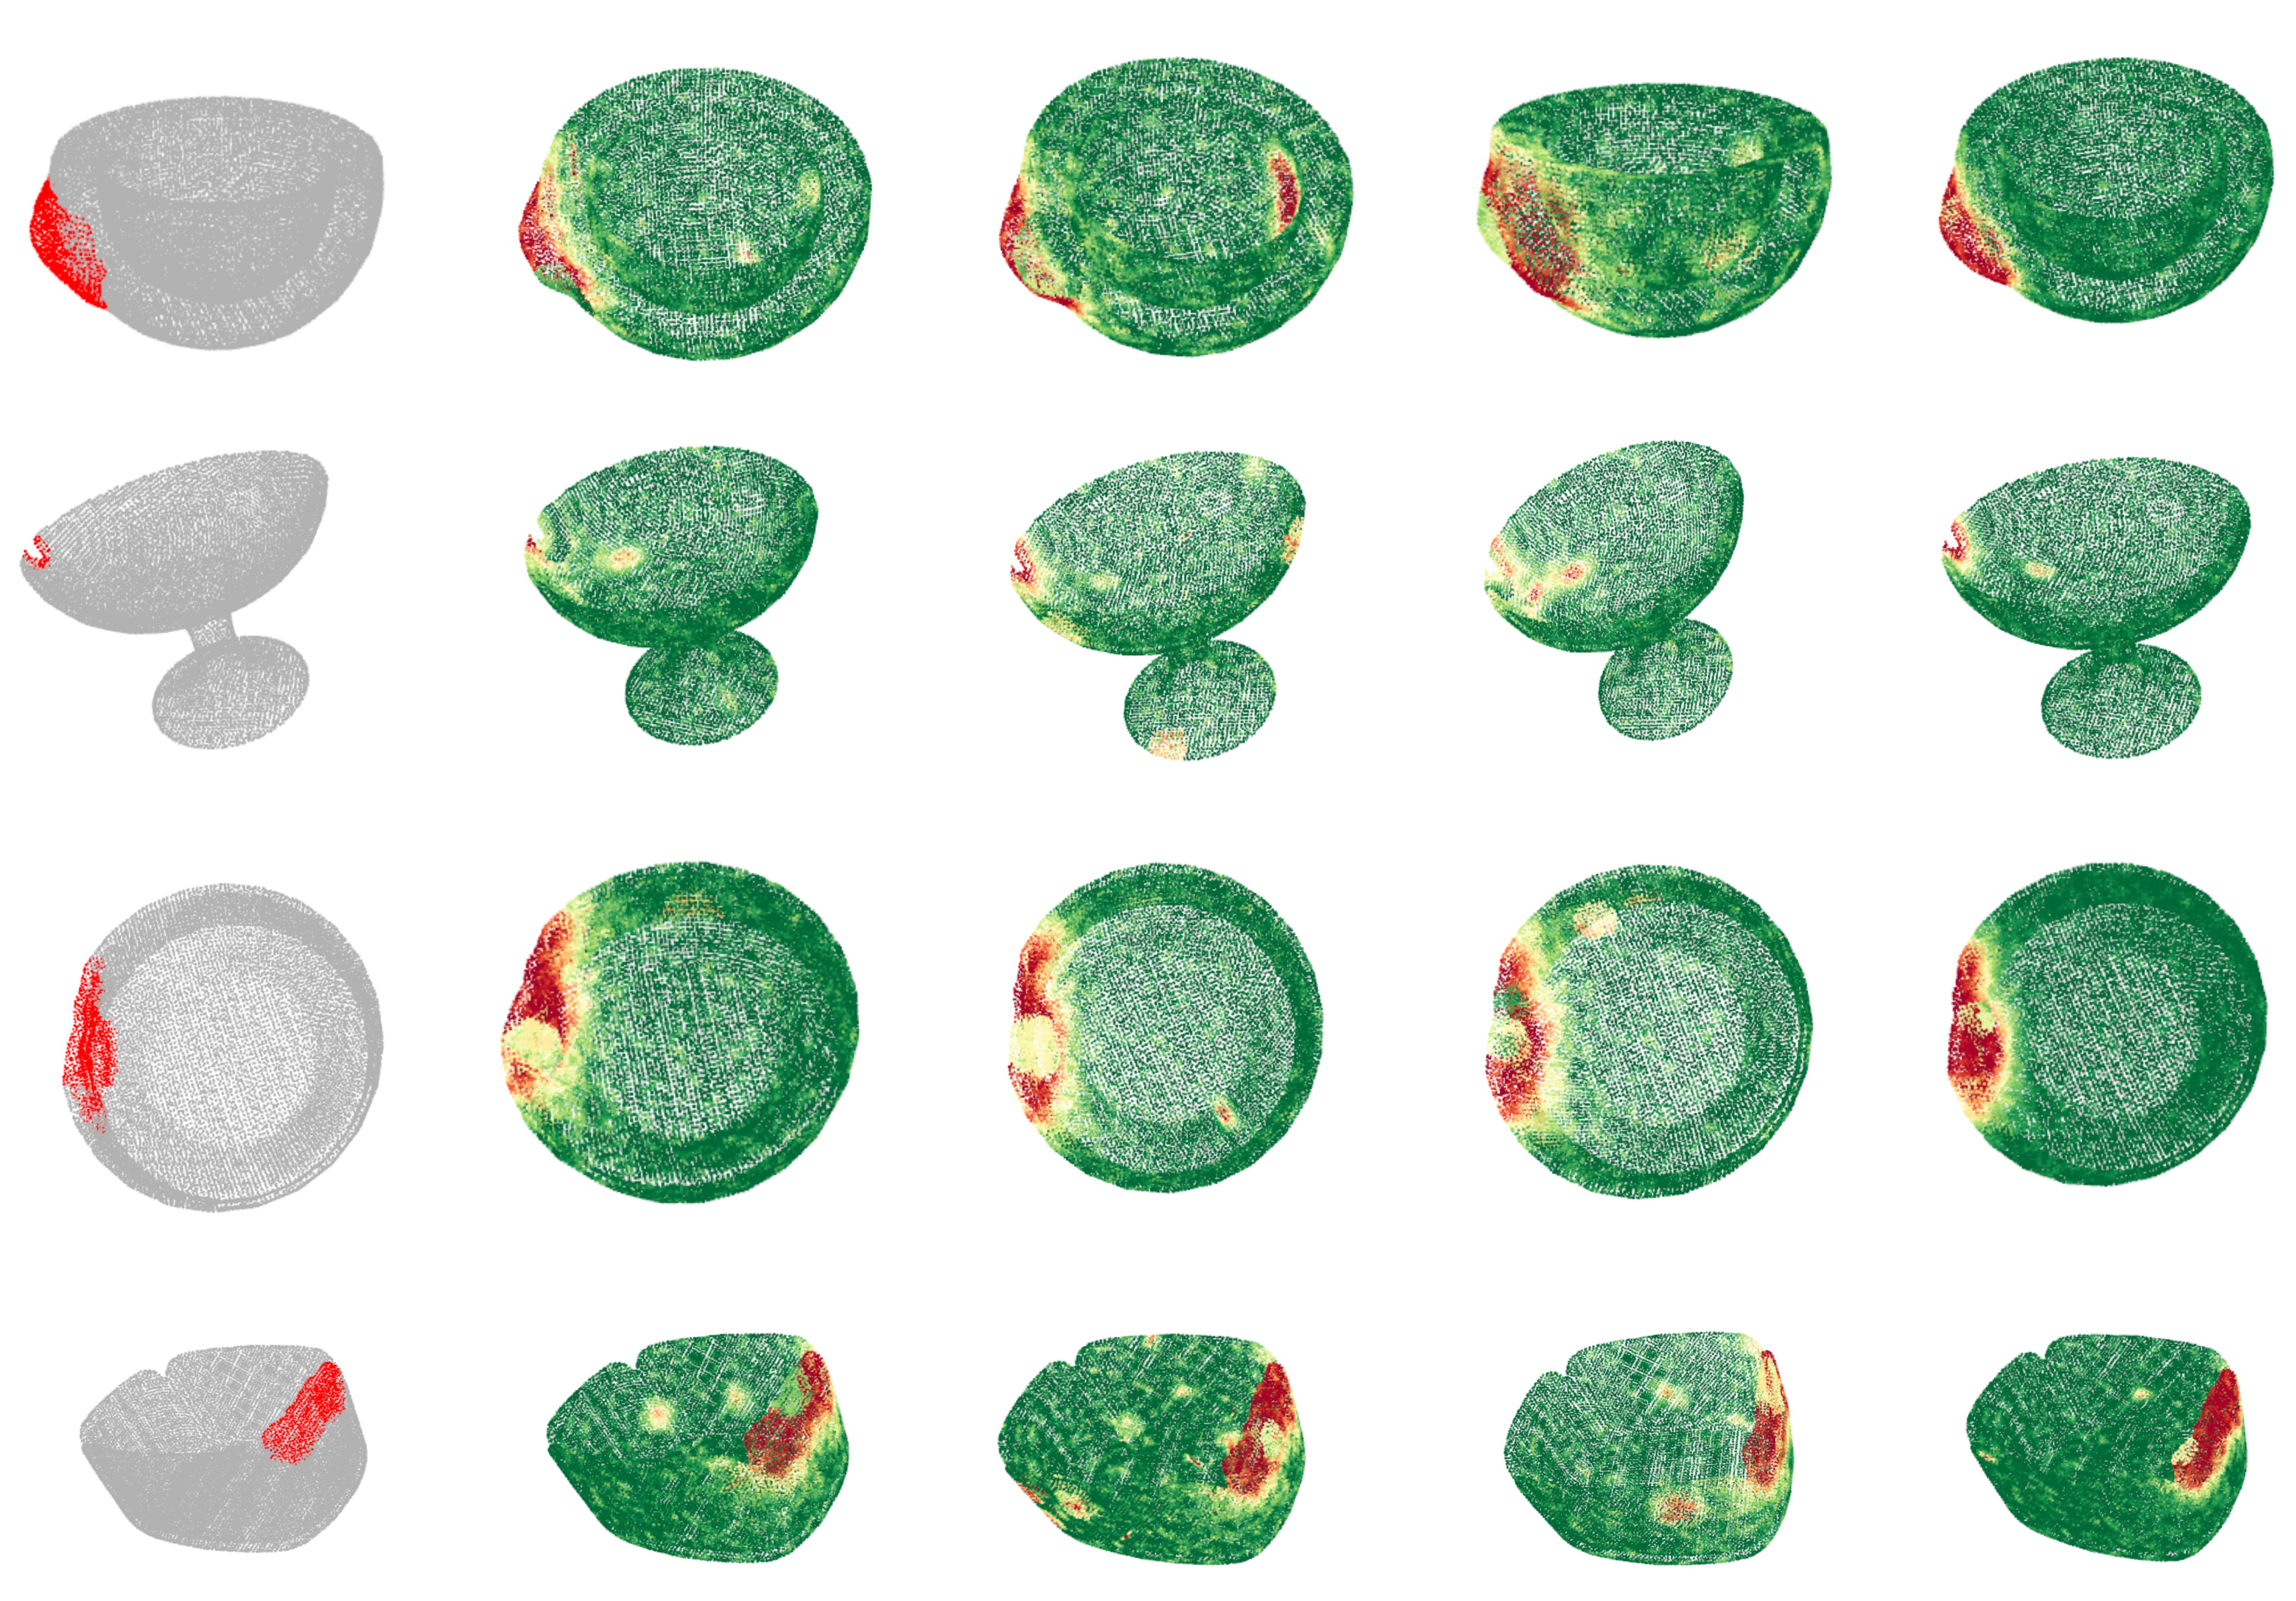
\includegraphics[width=\linewidth]{figs/shapenet}  
    Input + GT \hspace{1.2cm} 3D-ST \cite{bergmann2023anomaly} \hspace{1.3cm} Reg3D-AD \cite{liu2023real3d} \hspace{1.5cm} Group3AD   \cite{zhu2024towards} \hspace{1.7cm} Ours \hspace{0.8cm}
    \caption{Qualitative results on the newly collected Anomaly-ShapeNet \cite{li2024towards}. From left to right: input point clouds and ground truth annotations of anomalous points in red, and anomaly scores for each 3D point predicted by the proposed method.}
    \label{fig:shapenet}
\end{figure*}
%-------------------------------------------------------

\subsection{Result on Anomaly-ShapeNet}

%-------------------------------------------------------

\begin{table}[ht]
\centering
\caption{Average Result (\%) on Anomaly-ShapeNet dataset.}
\label{tab:ShapeNet}
\begin{tabular}{l|cc|cc|c}
\hline
& \multicolumn{2}{c|}{Point Level (\%)} & \multicolumn{2}{c|}{Object Level (\%)} & Speed \\
\hline
& AUROC & AUPR & AUROC & AUPR & FPS \\ 
\hline
BTF(Raw)                            & 55.2 & 16.4  & 49.5 & 57.4  & 2.09 \\ 
BTF(FPFH)                           & 63.0 & 21.0  & 53.1 & 61.0  & 1.16 \\ 
M3DM(PointMAE)                      & 61.8 & 21.5  & 55.4 & 61.4  & 0.31 \\ 
M3DM(PointBERT)                     & 60.3 & 19.5  & 53.7 & 59.6  & 0.52 \\ 
PatchCore(FPFH)                     & 58.2 & 21.1  & 57.1 & 61.0  & 0.10 \\ 
PatchCore(FPFH+Raw)                 & 60.4 & 22.3  & 58.6 & 63.2  & 0.10 \\ 
PatchCore(PointMAE)                 & 57.9 & 19.4  & 56.4 & 59.3  & 0.12 \\ 
Reg3D-AD \cite{liu2023real3d}       & 67.0 & 20.3  & 57.4 & 70.3  & 0.10 \\ 
3D-ST \cite{bergmann2023anomaly}    & 63.6 & 22.6  & 60.7 & 60.5  & 1.52 \\
Group3AD \cite{zhu2024towards}      & 84.6 & 25.4  & 81.4 & 95.3  & 2.55 \\ 
IMRNet \cite{li2024towards}         & 65.3 & 22.8  & 66.3 & 72.7  & 5.62 \\
R3D-AD \cite{zhou2024r3d}           & 75.1 & 23.7  & 75.2 & 73.6  & 7.15 \\
Ours                                & 91.2 & 38.7  & 86.8 & 98.7  & 17.31 \\
\hline
\end{tabular}
\end{table}
%-------------------------------------------------------

Table~\ref{tab:ShapeNet} and Figure~\ref{fig:shapenet} summarize our quantitative and qualitative results on Anomaly-ShapeNet. Our method attains a point-level AUROC of 91.2\% and point-level AUPR of 38.7\%, which improves over the strongest baseline, Group3AD, by 6.6\% and 13.3\%, respectively. At the object level our AUROC is 86.8\% and AUPR is 98.7\%, exceeding Group3AD by 5.4\% and 3.4\%. These accuracy gains are achieved alongside a large runtime advantage: our default configuration runs at 17.31 FPS on the RTX-3090 workstation, which is substantially faster than the competing methods listed in Table~\ref{tab:ShapeNet}. BTF(Raw) refers to the use of only the raw 3D coordinate features (x, y, z) within the Back-to-Front (BTF) framework \cite{horwitz2023back}. In contrast, BTF(FPFH) augments the same pipeline with Fast Point Feature Histograms (FPFH) \cite{rusu2009fast}. The entries M3DM(PointMAE) and M3DM(PointBERT) correspond to the model \cite{wang2023multimodal} configured to ignore its RGB branch and instead extract point cloud features with PointMAE \cite{pang2022masked} or PointBERT \cite{yu2022point}, respectively. For PatchCore variants, PatchCore(FPFH) replaces the usual ResNet-based feature extractor with FPFH descriptors \cite{rusu2009fast} before feeding them into the PatchCore anomaly scoring pipeline \cite{roth2022towards}. PatchCore(FPFH+Raw) further concatenates the raw spatial coordinates to each FPFH feature vector, and PatchCore(PointMAE) uses the PointMAE network \cite{pang2022masked} as the backbone feature extractor within the PatchCore framework.

The observed improvements can be traced to three design choices. First, multi-scale token fusion with the Mamba adapter aggregates complementary cues across Transformer layers so that subtle local deviations are evaluated in their broader geometric context. Defects such as bulges and concavities manifest across receptive fields and benefit from the cross-layer evidence that Mamba supplies. Second, the Geometric Semantic-Aware Sorter (GSAS) produces a geometry-preserving ordering that enables state-space fusion to propagate information along coherent surface trajectories rather than arbitrary token sequences. This geometric consistency reduces spurious contextual mixing and sharpens localization. Third, the selective anomalous feature generator provides localized, feature-space supervision that teaches the discriminator to attend to sparse, realistic deviations without corrupting global shape priors. Qualitatively, these components combine to produce compact heatmaps with low background noise for medium and large localized defects, as shown in Figure~\ref{fig:shapenet}. Failure modes are consistent with expectations for point-based pipelines. Very thin cracks that remove only a few points remain challenging and reduce AUPR because a small number of mis-scored points strongly affects precision. High-curvature ornamental details can sometimes be mistaken for defects, which suggests that future work could incorporate curvature-aware post-processing or augment the anomalous generator with structure-preserving perturbations. Overall, the results on Anomaly-ShapeNet demonstrate that the combination of GSAS, Mamba fusion, and sparse feature-space supervision yields both state-of-the-art detection and a deployment-friendly runtime.

\subsection{Result on Real3D-AD}

%-------------------------------------------------------
\begin{figure*}[!ht]
    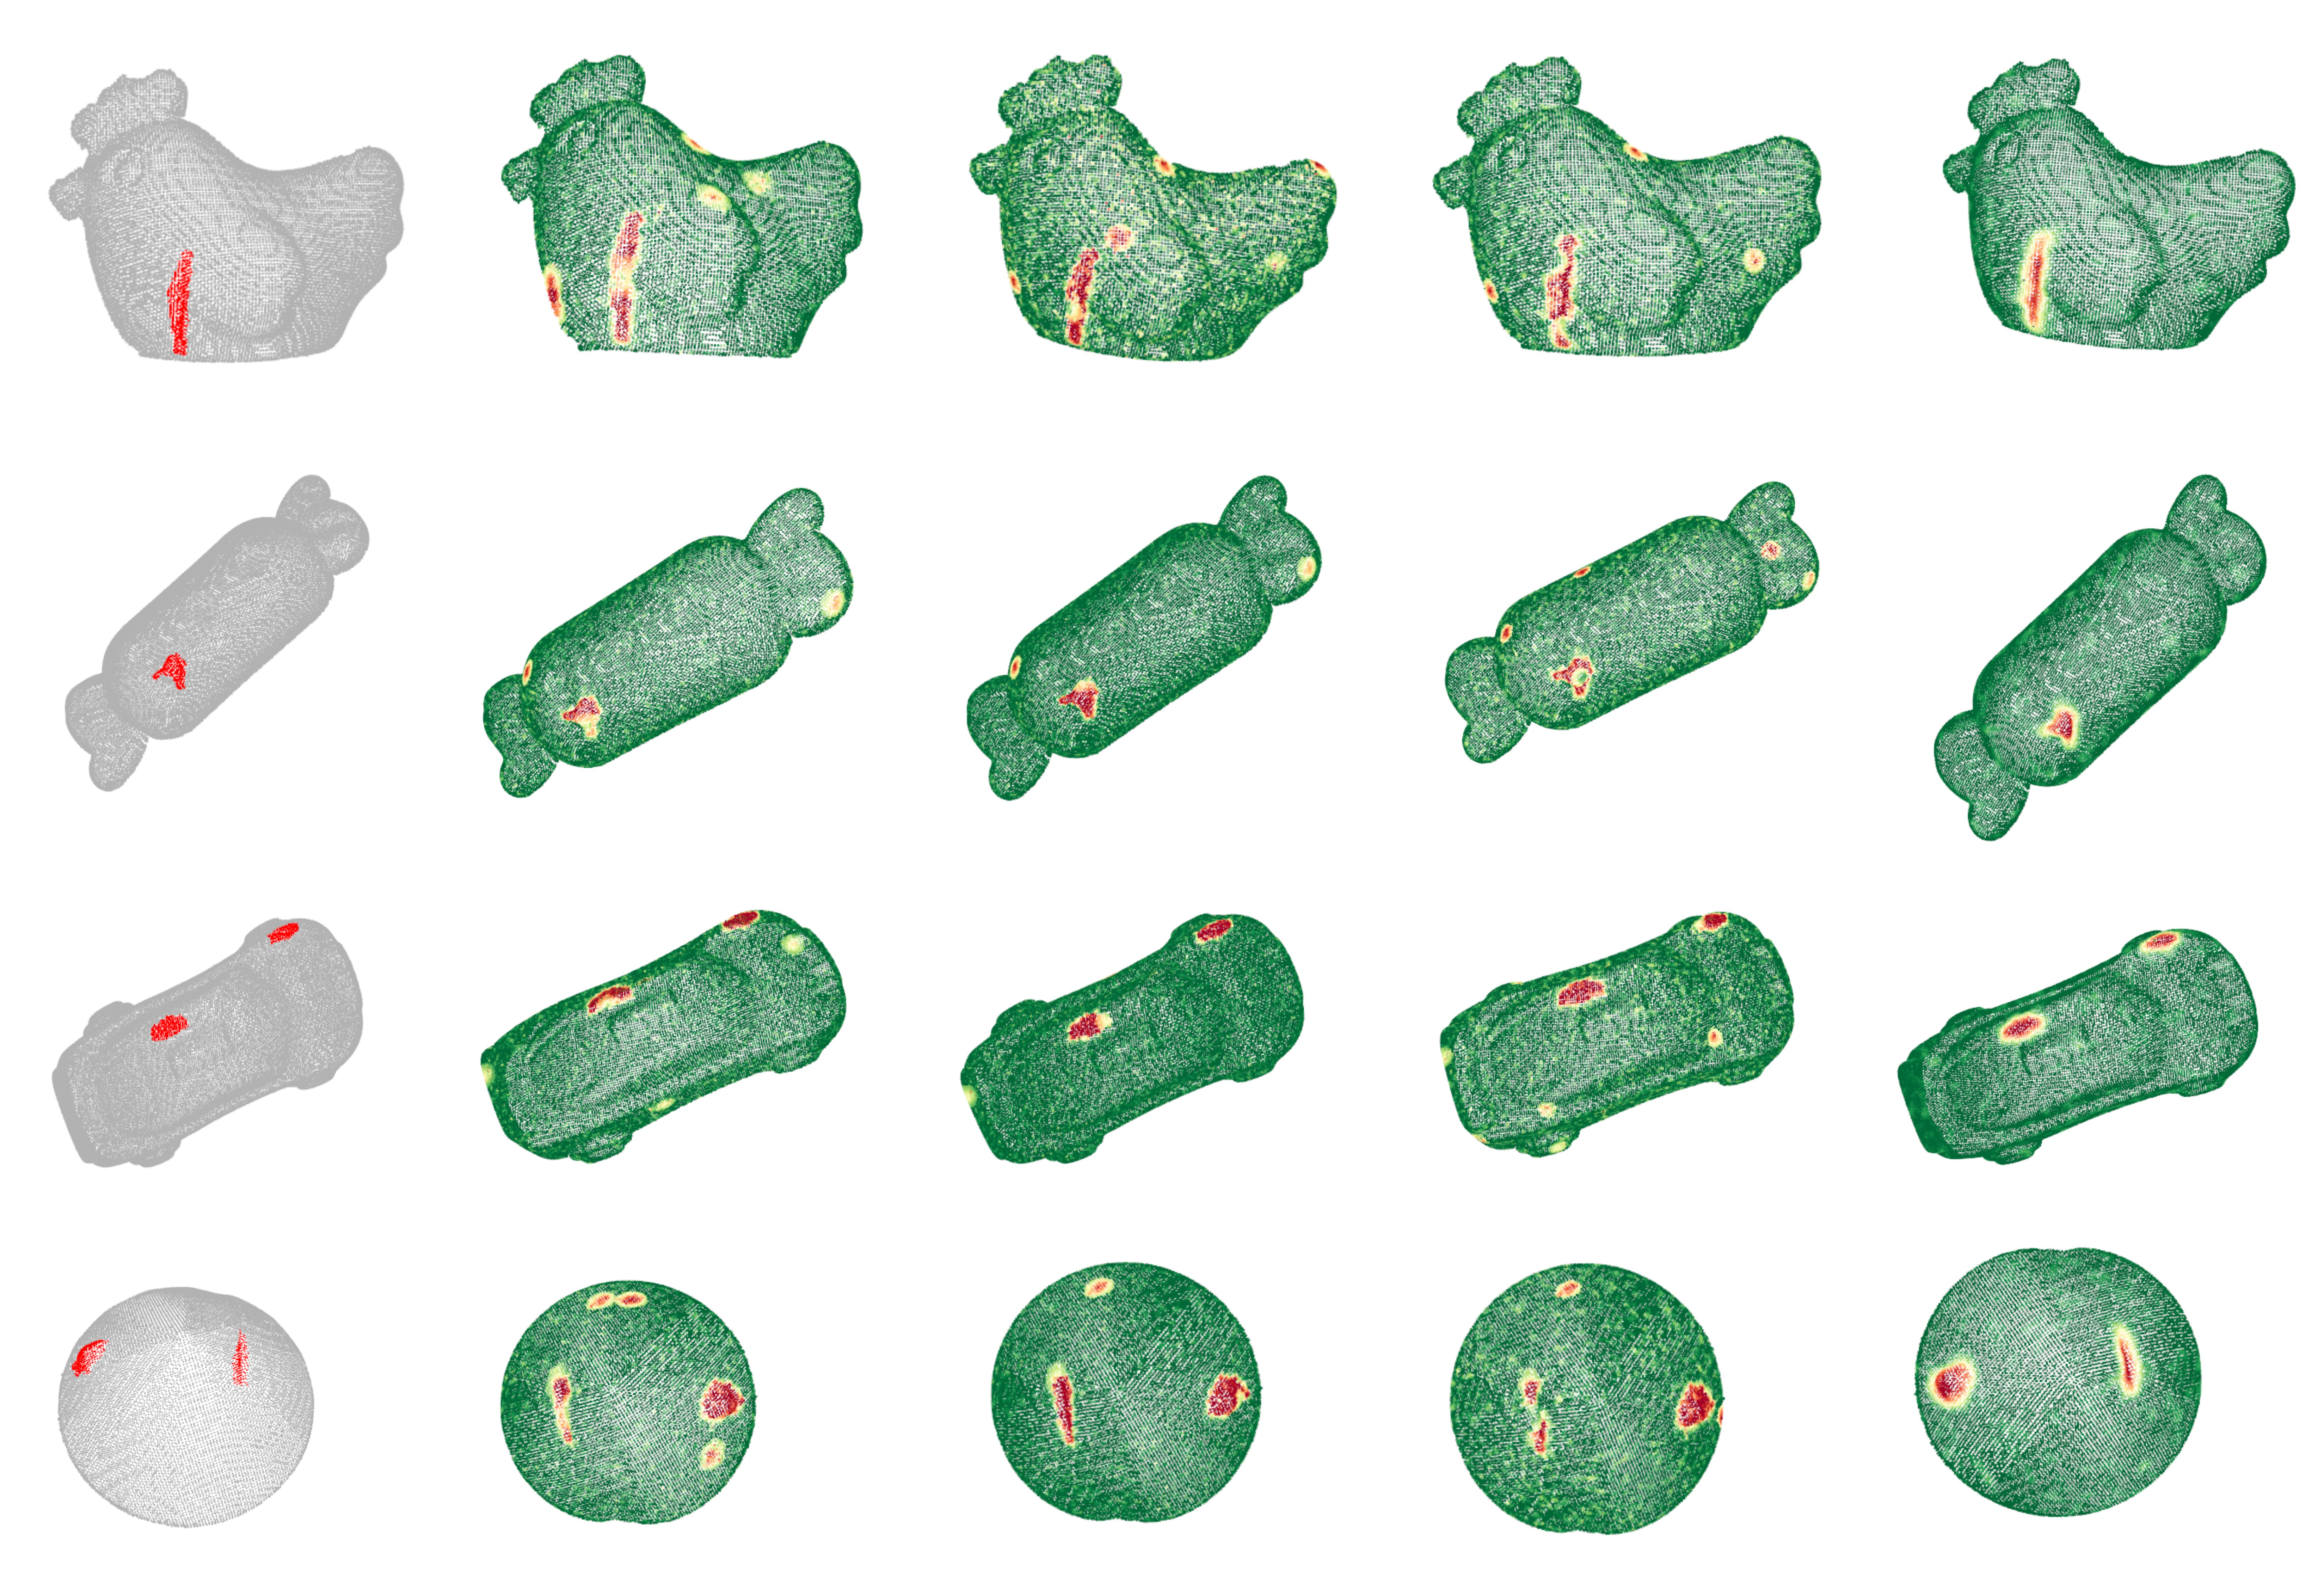
\includegraphics[width=\linewidth]{figs/real3d}
    Input + GT \hspace{1.2cm} 3D-ST \cite{bergmann2023anomaly} \hspace{1.3cm} Reg3D-AD \cite{liu2023real3d} \hspace{1.3cm} Group3AD   \cite{zhu2024towards} \hspace{1.7cm} Ours \hspace{1.5cm}
    \caption{Qualitative results on Real3D-AD dataset. From left to right: input point clouds, Ground truth annotations of anomalous points in red, and anomaly scores for each 3D point predicted by the proposed method.}
    \label{fig:real3d}
\end{figure*}
%-------------------------------------------------------

%-------------------------------------------------------

\begin{table}[ht]
\centering
\caption{Average Results (\%) on Real3D-AD dataset.}
\label{tab:Real3D}
\begin{tabular}{l|cc|cc|c}
\hline
& \multicolumn{2}{c|}{Point Level (\%)} & \multicolumn{2}{c|}{Object Level (\%)} & Speed \\
\hline
& AUROC & AUPR & AUROC & AUPR & FPS \\ 
\hline
BTF(Raw)                            & 57.3 & 2.4 & 60.5 & 61.3  & 2.05 \\
BTF(FPFH)                           & 73.2 & 6.6 & 63.7 & 61.6  & 1.01 \\
M3DM(PointMAE)                      & 63.9 & 4.9 & 55.4 & 57.5  & 0.31 \\
M3DM(PointBERT)                     & 63.9 & 5.4 & 54.0 & 58.3  & 0.52 \\
PatchCore(FPFH)                     & 57.9 & 7.3 & 59.6 & 59.3  & 0.10 \\
PatchCore(FPFH+Raw)                 & 68.2 & 12.5 & 68.4 & 66.9  & 0.10 \\
PatchCore(PointMAE)                 & 64.5 & 6.0 & 59.6 & 63.6  & 0.12 \\
Reg3D-AD \cite{liu2023real3d}       & 70.7 & 11.1 & 70.7 & 72.6  & 0.10 \\
3D-ST \cite{bergmann2023anomaly}    & 70.7 & 11.1 & 64.8 & 72.6  & 1.52 \\
Group3AD   \cite{zhu2024towards}    & 73.8 & 13.9 & 75.3 & 74.3  & 2.55 \\
IMRNet   \cite{li2024towards}       & 72.8 & 16.8 & 72.8 & 62.8  & 5.62 \\
R3D-AD   \cite{zhou2024r3d}         & 59.4 & 4.3 & 73.6 & 63.5  & 7.15 \\
Ours                                & 76.6 & 19.7 & 78.4 & 77.7 & 17.31 \\
\hline
\end{tabular}
\end{table}

%-------------------------------------------------------

Table~\ref{tab:Real3D} and Figure~\ref{fig:real3d} report performance on Real3D-AD, where scans are high density and defects arise under realistic sensor conditions. We compare with the same set of state-of-the-art methods used for Anomaly-ShapeNet. Our method achieves a point-level AUROC of 76.6\% and point-level AUPR of 19.7\%, improving over Group3AD by 2.8\% and 5.8\%, respectively. At the object level we obtain an AUROC of 78.4\% and an AUPR of 77.7\%, improving over Group3AD by 3.1\% and 3.4\%. As on the synthetic benchmark, our approach maintains a large throughput advantage with 17.31 FPS, which supports practical deployment in industrial inspection pipelines. Real3D-AD differs from synthetic benchmarks in three ways that highlight the strengths of our design. First, defects in real scans are often subtle and must be discriminated from sensor noise and varying point density. Mamba fusion aggregates multi-layer signals so that local irregularities are evaluated with respect to global part geometry, which reduces false positives caused by sensor artifacts. Second, GSAS ensures that the fusion operates on a surface-aware ordering, which is important in dense, complex scans to prevent unrelated surface regions from contaminating contextual cues. Third, the selective anomalous feature generator produces spatially sparse supervisory signals that encourage sensitivity to small but consistent deviations, which is useful when prototype sets are limited and supervised defect examples are scarce. Qualitatively, our method reliably highlights dents, missing material, and other geometric defects with high contrast while keeping false detections low in benign regions. Limitations include reduced sensitivity to appearance-only anomalies that do not affect geometry and occasional loss of localization precision in heavily occluded or extremely unevenly sampled areas. Practical mitigations include fusing appearance or reflectance channels when available and applying local density normalization during preprocessing. Results on Real3D-AD corroborate the conclusions from the synthetic benchmark. The combination of geometry-preserving ordering, linear-time cross-layer fusion, and sparse feature-space supervision improves both detection and localization robustness while offering a favorable runtime and memory profile for industrial applications.

\subsection{Ablation Study}

The ablation study aims to rigorously assess the contribution of each major component of the proposed framework. All results are averaged across the Anomaly-ShapeNet and Real3D-AD datasets to provide stable indicators of overall performance. Unless stated otherwise, the baseline configuration, denoted as Ours (full / baseline), employs a frozen Point-MAE backbone, the GSAS ordering module with Sinkhorn normalization (\(\tau=0.2\), 20 iterations), the Mamba state-space adapter with state dimension \(S=256\), a selective anomalous feature generator with corruption probability \(p=0.05\) and Gaussian noise \(\sigma=0.1\), and a single-layer multi-head attention discriminator. The reported speed corresponds to end-to-end inference throughput measured under identical hardware conditions.

Table~\ref{tab:backbone_ablation} presents the results for different backbone training strategies. The frozen backbone represents the baseline configuration used throughout this paper. In the fine-tuning variant, the backbone weights are updated with a reduced learning rate equal to one-tenth of that of the adapter and discriminator, while all other settings remain unchanged. The scratch variant initializes the backbone randomly and doubles the number of training epochs to allow sufficient convergence. The results show that the pretrained backbone is indispensable. Fine-tuning provides a slight gain in AUROC and AUPR at both the point and object levels, likely due to improved alignment of pretrained features with the target domain. Training from scratch, however, leads to a drastic performance drop, confirming that the backbone pretraining provides fundamental representational priors that cannot be recovered solely through synthetic-negative supervision.

\begin{table}[ht]
\centering
\caption{Backbone ablation results averaged across the two datasets.}
\label{tab:backbone_ablation}
\begin{tabular}{l|cc|cc|c}
\hline
& \multicolumn{2}{c|}{Point Level (\%)} & \multicolumn{2}{c|}{Object Level (\%)} & Speed \\
\hline
& AUROC & AUPR & AUROC & AUPR & FPS \\  
\hline
Frozen (Ours, baseline) & 83.9 & 29.2 & 82.6 & 88.2 & 17.3 \\
Fine-tune backbone (last-to-all) & 85.3 & 32.2 & 83.6 & 89.7 & 17.3 \\
Train from scratch & 71.9 & 21.2 & 72.6 & 68.2 & 17.3 \\
\hline
\end{tabular}
\end{table}

Table~\ref{tab:gsas_ablation} examines the effectiveness of the geometry- and semantics-aware sorting provided by the GSAS module. The GSAS ordering transforms unordered point tokens into a structured sequence suitable for the Mamba adapter. Removing GSAS entirely (no ordering) or randomly permuting tokens severely degrades both point- and object-level detection, indicating that sequence-aware context propagation without structural coherence fails to capture consistent semantics. Sorting tokens deterministically by spatial coordinates recovers part of the performance but remains notably inferior to the learned GSAS ordering, suggesting that GSAS learns more meaningful relationships than can be achieved by geometric sorting alone. The slight increase in frames per second (FPS) observed when GSAS is disabled confirms that the ordering step constitutes the primary computational overhead. Nonetheless, the accuracy gains justify its inclusion for practical deployments.

\begin{table}[ht]
\centering
\caption{Ordering (GSAS) ablation results averaged across the two datasets.}
\label{tab:gsas_ablation}
\begin{tabular}{l|cc|cc|c}
\hline
& \multicolumn{2}{c|}{Point Level (\%)} & \multicolumn{2}{c|}{Object Level (\%)} & Speed \\
\hline
& AUROC & AUPR & AUROC & AUPR & FPS \\  
\hline
GSAS (Ours, baseline) & 83.9 & 29.2 & 82.6 & 88.2 & 17.3 \\
No GSAS (no ordering) & 67.0 & 15.0 & 61.0 & 60.0 & 20.5 \\
Random ordering & 65.5 & 14.0 & 60.0 & 59.0 & 20.5 \\
Coordinate-sorted & 75.5 & 22.0 & 71.0 & 69.5 & 18.5 \\
\hline
\end{tabular}
\end{table}

The role of the Sinkhorn-based soft permutation mechanism within GSAS is analyzed in Table~\ref{tab:sinkhorn_ablation}. This mechanism enforces an approximately doubly stochastic transport matrix that allows gradients to propagate effectively during training. Replacing it with a hard Hungarian assignment preserves assignment fidelity but removes differentiability, resulting in minor performance degradation during end-to-end learning. Omitting the Sinkhorn normalization and using a simple softmax over affinities produces the weakest results, as this configuration allows overlapping or diffuse assignments that diminish spatial and semantic distinctness. These results verify that the Sinkhorn operator strikes a favorable balance between optimization stability and structural regularity, which is essential for coherent feature alignment.

\begin{table}[ht]
\centering
\caption{Permutation (Sinkhorn) ablation results averaged across the two datasets.}
\label{tab:sinkhorn_ablation}
\begin{tabular}{l|cc|cc|c}
\hline
& \multicolumn{2}{c|}{Point Level (\%)} & \multicolumn{2}{c|}{Object Level (\%)} & Speed \\
\hline
& AUROC & AUPR & AUROC & AUPR & FPS \\  
\hline
Sinkhorn (Ours, baseline) & 83.9 & 29.2 & 82.6 & 88.2 & 17.3 \\
Hard Hungarian (discrete) & 82.0 & 28.0 & 81.0 & 86.5 & 16.0 \\
Softmax (no Sinkhorn) & 78.5 & 24.0 & 76.0 & 80.0 & 17.8 \\
\hline
\end{tabular}
\end{table}

Table~\ref{tab:adapter_ablation} compares the proposed Mamba state-space adapter to alternative sequence modeling mechanisms. The Mamba adapter propagates contextual information linearly in sequence order with low memory and computational overhead. A transformer-based attention module achieves slightly higher accuracy, yet its computational cost and latency are significantly higher. The per-token MLP variant, which lacks explicit inter-token interactions, and the identity variant, which omits the adapter entirely, both show marked decreases in accuracy. These observations confirm that efficient long-range context modeling is crucial for discriminating subtle anomalies that depend on relational cues across spatially distant patches. The Mamba adapter achieves a strong balance between accuracy and efficiency, making it suitable for real-time industrial inspection scenarios where computational resources are limited.

\begin{table}[ht]
\centering
\caption{Adapter ablation results averaged across the two datasets. Memory and FLOPs correspond to approximate end-to-end inference measurements.}
\label{tab:adapter_ablation}
\begin{tabular}{l|cc|cc|c|cc}
\hline
& \multicolumn{2}{c|}{Point Level (\%)} & \multicolumn{2}{c|}{Object Level (\%)} & Speed & Mem & FLOPs \\
\hline
& AUROC & AUPR & AUROC & AUPR & FPS & (GB) & (GFLOP) \\  
\hline
Mamba (Ours, baseline) & 83.9 & 29.2 & 82.6 & 88.2 & 17.3 & 3.2 & 120 \\
Attention (2 layers, full self-attn) & 85.0 & 33.0 & 84.5 & 90.0 & 9.2 & 6.8 & 260 \\
MLP (per-token, 2 layers) & 78.0 & 22.0 & 75.0 & 80.0 & 18.5 & 3.0 & 95 \\
Identity (no adapter) & 74.5 & 18.0 & 72.0 & 76.5 & 19.8 & 2.8 & 70 \\
\hline
\end{tabular}
\end{table}

Finally, Table~\ref{tab:afg_ablation} investigates the effect of the anomalous feature generator and its corruption density. The selective sparse corruption used in the baseline introduces stochastic perturbations to approximately five percent of tokens, producing localized, hard negative examples. The dense corruption variant perturbs all tokens uniformly. The results clearly show that sparse corruption leads to superior AUROC and AUPR, particularly at the object level, confirming that the network benefits from learning localized deviations rather than global distortions. Dense corruption reduces performance because it drives the model to focus on global statistical shifts rather than spatially constrained anomalies, thereby diminishing its sensitivity to real defects. This experiment validates the design choice of sparse corruption as a simple yet effective mechanism for approximating the local nature of physical anomalies.

\begin{table}[ht]
\centering
\caption{Anomalous feature generator (AFG) ablation results averaged across the two datasets.}
\label{tab:afg_ablation}
\begin{tabular}{l|cc|cc|c}
\hline
& \multicolumn{2}{c|}{Point Level (\%)} & \multicolumn{2}{c|}{Object Level (\%)} & Speed \\
\hline
& AUROC & AUPR & AUROC & AUPR & FPS \\  
\hline
Selective sparse corruption (p=0.05, Ours) & 83.9 & 29.2 & 82.6 & 88.2 & 17.3 \\
Dense corruption (p=1.0) & 79.0 & 20.5 & 78.0 & 82.0 & 17.3 \\
\hline
\end{tabular}
\end{table}

Collectively, these ablations highlight the functional importance of each proposed component. The pretrained backbone and GSAS ordering form the structural foundation of the framework, while the Sinkhorn normalization ensures stable and meaningful token assignments. The Mamba adapter provides efficient and scalable long-range context propagation with minimal accuracy loss compared to attention-based models, and the selective sparse corruption strategy effectively mimics realistic anomaly distributions. These findings substantiate the architectural design choices and demonstrate the balance achieved between accuracy, interpretability, and computational efficiency.

\section{Conclusion}

In this work, we introduced a compact and practical framework for 3D industrial defect detection that combines a Geometric Semantic-Aware Sorter (GSAS), a Mamba state-space adapter, and an attention-based discriminator trained with sparse feature-space pseudo-anomalies. GSAS produces a differentiable, surface-consistent soft-ordering of multi-layer per-patch tokens so that sequence models can operate on geometry-preserving token trajectories. The Mamba adapter then fuses the ordered slots with a linear-time state-space recurrence to inject long-range, cross-layer context with minimal parameter overhead. The attention-based discriminator operates on the fused slots and produces slot-level anomaly logits that are reprojected to points for dense localization. The entire pipeline is designed to be parameter-efficient: the large pretrained Transformer backbone remains frozen and only lightweight adapters and heads are trained.

Empirically, the proposed pipeline establishes a new operating point for accurate and efficient 3D anomaly localization. On the synthetic Anomaly-ShapeNet benchmark our method attains a point-level AUROC of 91.2\% and AUPR of 38.7\%, and achieves an object-level AUROC of 86.8\% with object-level AUPR 98.7\%. These results improve upon the strongest prior competitor (Group3AD) by +6.6 percentage points in point-level AUROC (91.2 vs. 84.6) and by +13.3 percentage points in point-level AUPR (38.7 vs. 25.4); object-level gains are +5.4 AUROC and +3.4 AUPR. On the high-fidelity Real3D-AD benchmark our method achieves a point-level AUROC of 76.6\% and AUPR 19.7\%, and an object-level AUROC/AUPR of 78.4\%/77.7\%, corresponding to improvements over Group3AD of +2.8 (point AUROC), +5.8 (point AUPR), +3.1 (object AUROC) and +3.4 (object AUPR) percentage points. Beyond accuracy, our implementation runs at roughly 17.3 FPS, which is approximately 6.8$\times$ faster than Group3AD in the reported configuration, demonstrating favorable trade-offs between accuracy and runtime. Ablation studies corroborate that GSAS, Mamba fusion, and the selective feature-space supervision each contribute substantially to localization quality and robustness to noise and sampling density

For future work, we plan to (i) investigate cross-modal extensions that incorporate RGB or reflectance where available, (ii) explore hierarchical or adaptive slot constructions to further scale to extremely large scans, and (iii) develop online adaptation strategies for continual deployment in industrial inspection pipelines. We believe the proposed combination of GSAS, Mamba, and selective supervision provides a strong foundation for scalable, interpretable, and real-time 3D anomaly detection.


%%%%%%%%%%%%%%%%%%%%%%%%%%%%%%%%%%%%%%%%%%%%%%%%%%%%%%%%%%%%%%%%%%%%%%

% Main text
%\section{Intro}\label{intro}

% Numbered list
% Use the style of numbering in square brackets.
% If nothing is used, default style will be taken.
%\begin{enumerate}[a)]
%\item 
%\item 
%\item 
%\end{enumerate}  

% Unnumbered list
%\begin{itemize}
%\item 
%\item 
%\item 
%\end{itemize}  

% Description list
%\begin{description}
%\item[]
%\item[] 
%\item[] 
%\end{description}  

% Figure
%\begin{figure}[<options>]
%	\centering
%		\includegraphics[<options>]{}
%	  \caption{}\label{fig1}
%\end{figure}


%\begin{table}[<options>]
%\caption{}\label{tbl1}
%\begin{tabular*}{\tblwidth}{@{}LL@{}}
%\toprule
%  &  \\ % Table header row
%\midrule
% & \\
% & \\
%& \\
% & \\
%\bottomrule
%\end{tabular*}
%\end{table}

% Uncomment and use as the case may be
%\begin{theorem} 
%\end{theorem}

% Uncomment and use as the case may be
%\begin{lemma} 
%\end{lemma}

%% The Appendices part is started with the command \appendix;
%% appendix sections are then done as normal sections
%% \appendix

%\section{Method}\label{method}

% To print the credit authorship contribution details
%\printcredits

%% Loading bibliography style file
%\bibliographystyle{model1-num-names}
\bibliographystyle{elsarticle-num}
%\bibliographystyle{cas-model2-names}

% Loading bibliography database
\bibliography{cas-refs}

% Biography
%\bio{}
% Here goes the biography details.
%\endbio

%\bio{pic1}
% Here goes the biography details.
%\endbio

\end{document}


